








%%% Here is the class with everything we need, if you don't want, you don't have to take a look at it, as it will probably cover your needs by far. These three options are used after the class article, which this template is based in.
% Twoside will act as an special parameter, because if the document is twosided indeed, headers and footers will be adapted in consequence.
% I recently added the language parameter to change it more easily, so the label of all theorems are redefined accordingly, depending on which is used. Disclaimer: only available for Catalan, English and Spanish. If no language is selected, English is enforced.


% \documentclass[a4paper,12pt,oneside,catalan]{all-in-one} %% ONESIDE
\documentclass[a4paper,12pt,twoside,english]{all-in-one} %% TWOSIDE

% Here is the font I usually use, it can be changed of course.
% In that case, these next two lines have to be deleted.
\usepackage{ebgaramond}
% Equations have the same font.
\usepackage[cmintegrals,cmbraces,ebgaramond]{newtxmath}

\doctitle{Software Tools and Techniques}
\docsubtitle{Condensed Lab Report (Lab 1 to Lab4)}

\author{Chavda Haarit Ravindrakumar \\ \texttt{23110077}}

% A text that goes into the footer. You can even include a logo. It can be left blank, too.
%% Option 1: \footext{
\includegraphics[width=2em]{titlepage.png}}
%% Option 2: \footext{\copyright\ \the\year by Cookie Monster}
% What I usually use: 
\footext{}

% Don't comment the command below if it's not of much inconvenience, please!
\greetings
% Licensing on every page? Comment if you don't want it.
% \licensing

% Last things
% This is my favourite config for bibliography. Each one of the references can be briefly explained with the field "note".
\RequirePackage[style=english]{csquotes}
\RequirePackage[
backend=biber,
style=alphabetic,
sorting=ynt
]{biblatex}
\newcommand{\familynameformat}[1]{\MakeUppercase{#1}}
\AtBeginBibliography{%
  \renewcommand{\mkbibnamefamily}{\familynameformat}%
}
\renewbibmacro*{begentry}{%
  \iffieldundef{note}
    {\undef\bbxnote}
    {\savefield{note}{\bbxnote}%
     \clearfield{note}}}
\renewbibmacro*{finentry}{%
  \restorefield{note}{\bbxnote}%
  \iffieldundef{note}
    {\finentry}
    {\setunit{\finentrypunct\par\vspace{\bibitemsep}\nobreak}
     \textit{\printfield{note}}%
     \finentry}}
\let\familynameformat=\textsc
\nocite{*}

\addbibresource{bibl.bib}


% Hyperref always required last one.
\RequirePackage{hyperref}
\makeatletter
\hypersetup{%
  hidelinks,
  pdfstartview=Fit,%
  pdfmenubar=true,%
  pdftoolbar=true,%
  bookmarksopen=false,%
  pdftitle={\@docsubtitle},%
  pdfauthor={\templateauthor},%
  pdfsubject={\@doctitle},%
  pdflang={\languagename},%
  pdfkeywords={mathematics},%
  pdfproducer={pdfTeX}}
\makeatother

% Setting up the titlepage.
\makeatletter%
\title{{\large\textit{\@doctitle}}\\[0.5cm]{\Huge\color{gray}\textsc{\@docsubtitle}}}%
\makeatother%
\date{\today}

% Dummy text
\usepackage{lipsum}

\begin{document}
% Interlineate, it can be changed.
\setlength{\baselineskip}{.70cm}

\begin{titlepage}
\maketitle\vfill
% \centering
\includegraphics[width=20em]{titlepage.png}
% \doclicenseThis
% Very important, regarding page numbering. Keep in mind differences between oneside and twoside
\thispagestyle{empty}
\end{titlepage}

% Table of contents
\thispagestyle{plain}
\tableofcontents
\newpage

\pagestyle{\defaultsettings}

\section{Lab 01}
\subsection{Introduction and Concepts}
Lab 01 is designed to introduce the fundamentals of version control systems (VCS), focusing on practical, hands-on tasks using Git and GitHub. In this lab, we will explore the basics of these tools, which are essential for efficiently managing and maintaining project development workflows. Additionally, the lab covers GitHub Actions, a powerful framework that enables automated Continuous Integration (CI) and Continuous Deployment (CD) processes.

Key Concepts
What is a Version Control System (VCS)?
A version control system is a tool that helps track changes to files over time, allowing multiple people to work on a project collaboratively and manage revisions easily. It enables developers to revert to previous versions, compare changes, and resolve conflicts when multiple contributors edit the same files.

What is CI/CD?
Continuous Integration (CI) is the practice of automatically building and testing code every time changes are committed, ensuring that integrations happen frequently and errors are caught early. Continuous Deployment (CD) refers to the automated process of delivering code changes to production quickly and safely, reducing manual intervention in releasing updates and new features.

\subsection{Tools and Setup}
Manjaro Linux was used as the operating system, which has Git pre-installed by default. If Git is not already available, it can be installed on Manjaro by running:
"sudo pacman -S git base-devel"
For Continuous Integration (CI) and Continuous Deployment (CD), the setup included the use of the Pylint GitHub Action. This tool automatically checks Python code quality as part of the CI/CD workflow on GitHub, ensuring standards are maintained and potential errors are caught early.



\subsection{Methodology and Execution}

The initial step involves configuring Git with user credentials. The following commands are used to set the global username and email:

\begin{figure}[H]
    \centering
    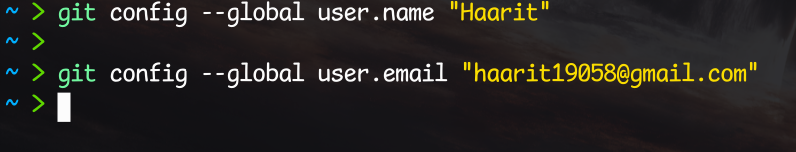
\includegraphics[width=0.75\linewidth]{image01.png}
    \caption{setting up git}
    \label{fig:placeholder}
\end{figure}

We have to tell git that the directory is safe or not and therefore git maintains a list of safe directories. We can ommit that part by piping the main command into grep -v safe.directories.
To verify the configuration, use:
\begin{figure}[H]
    \centering
    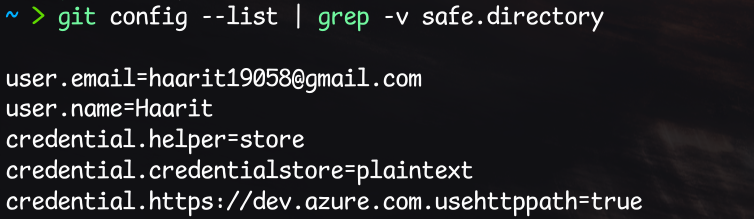
\includegraphics[width=0.75\linewidth]{image02.png}
    \caption{Verify the configurations}
    \label{fig:placeholder}
\end{figure}


Next, a new project directory called lab1 is created and navigate to that folder:
\begin{figure}[H]
    \centering
    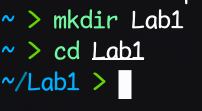
\includegraphics[width=0.4\linewidth]{image03.png}
    \caption{make new directory}
    \label{fig:placeholder}
\end{figure}

The Git repository is then initialized in the folder, and a README file is created with a brief description:
\begin{figure}[H]
    \centering
    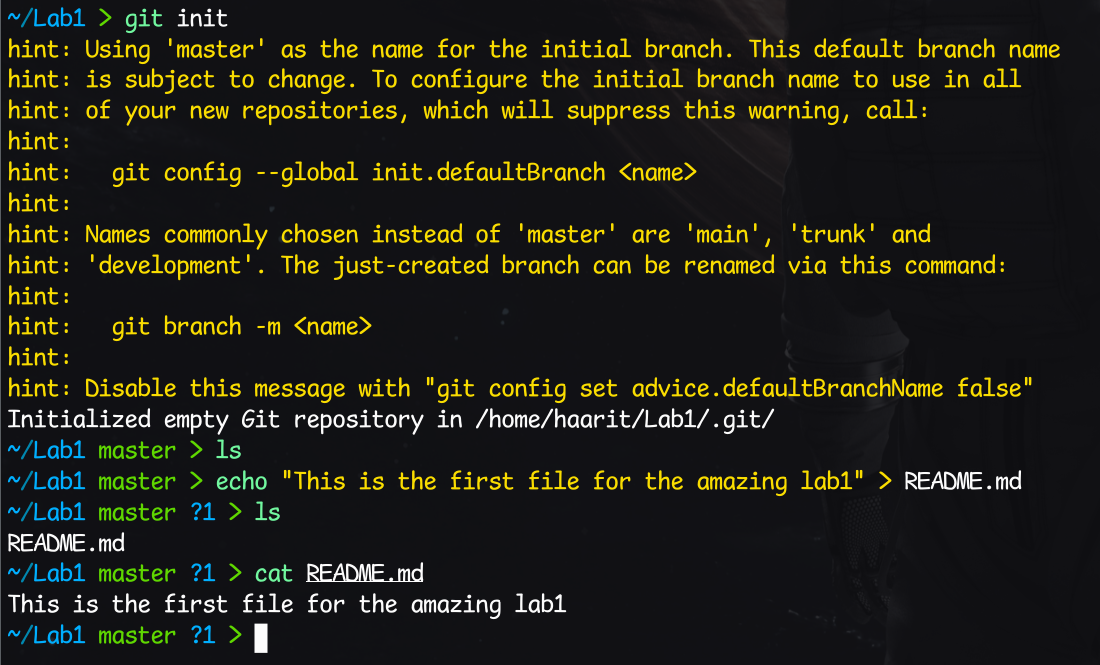
\includegraphics[width=0.75\linewidth]{image04.png}
    \caption{initializing and adding readme}
    \label{fig:placeholder}
\end{figure}



The README file is added to the staging area, either by adding all files or just the README 
specifically:
\begin{itemize}
    \item git add .           # Adds all files
    \item git add README.md   # Adds only the README file
\end{itemize}
\begin{figure}[H]
    \centering
    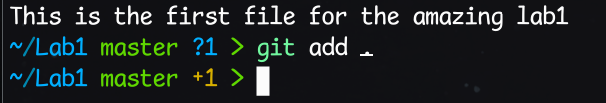
\includegraphics[width=0.5\linewidth]{image05.png}
    \caption{Adding the readme file to staging area}
    \label{fig:placeholder}
\end{figure}


After staging, the first commit is made with an appropriate message: git commit -m "First commit of the course"

\begin{figure}[H]
    \centering
    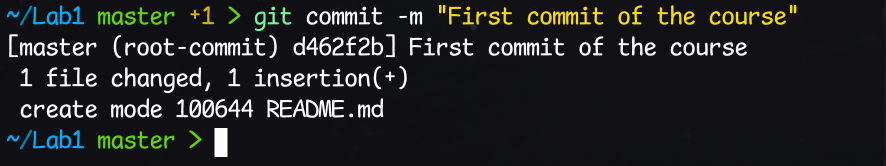
\includegraphics[width=0.5\linewidth]{image06.png}
    \caption{First commit msg}
    \label{fig:placeholder}
\end{figure}



The history of commits can be viewed with: git log
\begin{figure}[H]
    \centering
    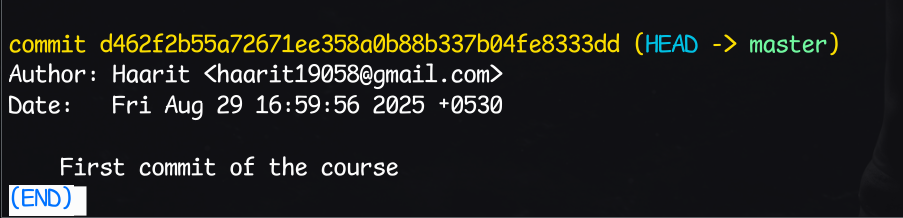
\includegraphics[width=0.75\linewidth]{image07.png}
    \caption{Seeing the log}
    \label{fig:placeholder}
\end{figure}


Creating a remote repository by following the steps shown in the figures ..

Go to github.com, sign in with your email id and ther will be a green button which says "new" and click that button to create a new repository.

\begin{figure}[H]
    \centering
    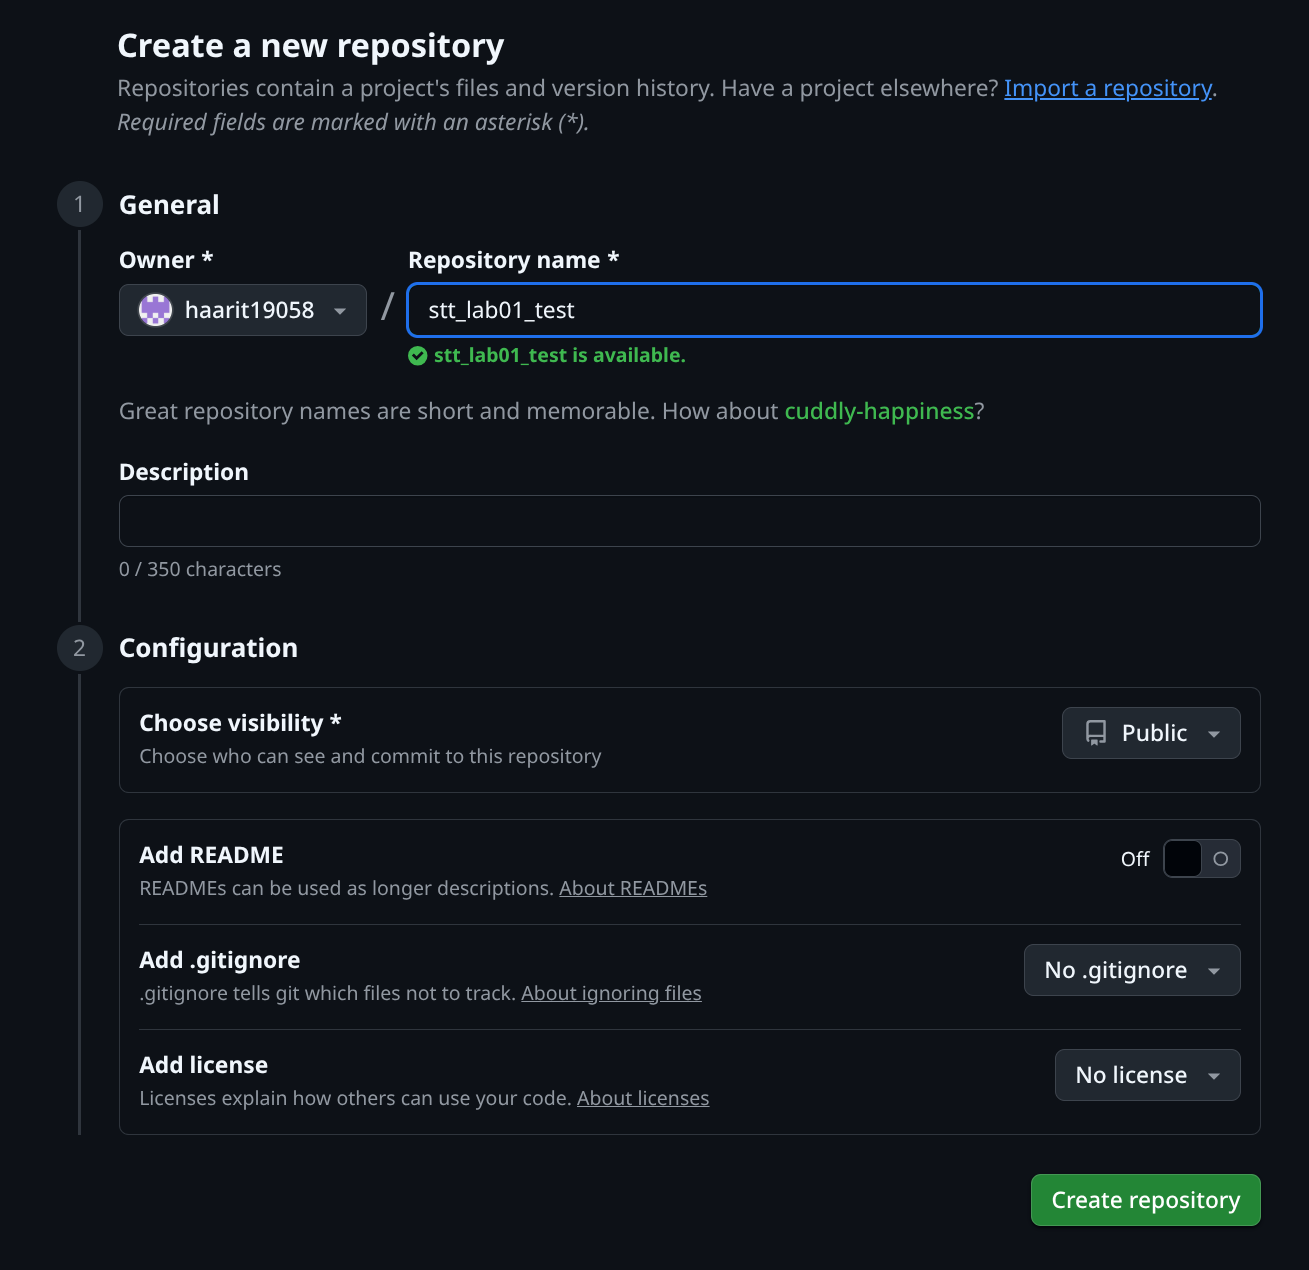
\includegraphics[width=0.75\linewidth]{image08.png}
    \caption{Creating a new repo..}
    \label{fig:placeholder}
\end{figure}



To connect the local repository to GitHub, a remote repository named STT is created on GitHub. The current branch is renamed to main for consistency with GitHub standards, and the remote repository is linked:

The github uses as main as its master branch and git uses master as default branch so we need to change the name of default branch form master to main using : git branch -M main

Now add the remote repo URL and link it with the local repository: \\
\texttt{git remote add origin https://github.com/haarit19058/stt\_lab01\_test.git}


Use git remote -v to see the remote repository link


\begin{figure}[H]
    \centering
    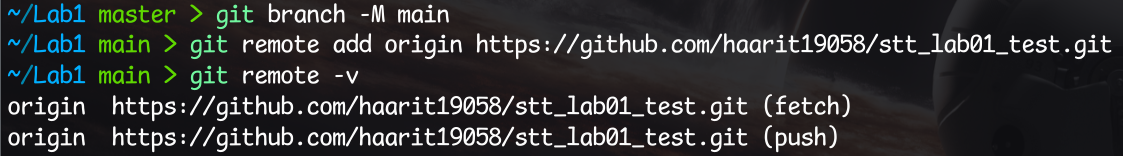
\includegraphics[width=0.75\linewidth]{image09.png}
    \caption{linking with remote repository}
    \label{fig:placeholder}
\end{figure}

Push the commits to the remote branch and set the default upstream using these commands : git push --set-upstream origin main
\begin{figure}[H]
    \centering
    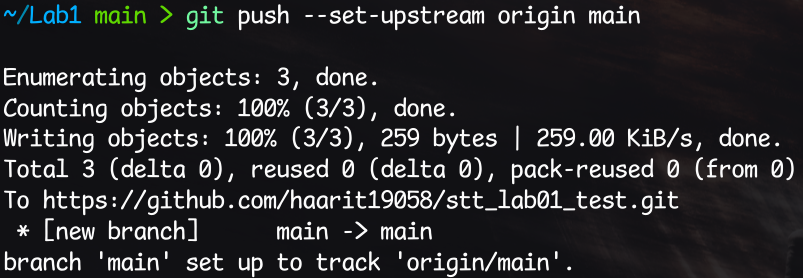
\includegraphics[width=0.75\linewidth]{image10.png}
    \caption{push the changes to remote repo and set the upstream}
    \label{fig:placeholder}
\end{figure}


Cloning a existing repository :
\begin{figure}[H]
    \centering
    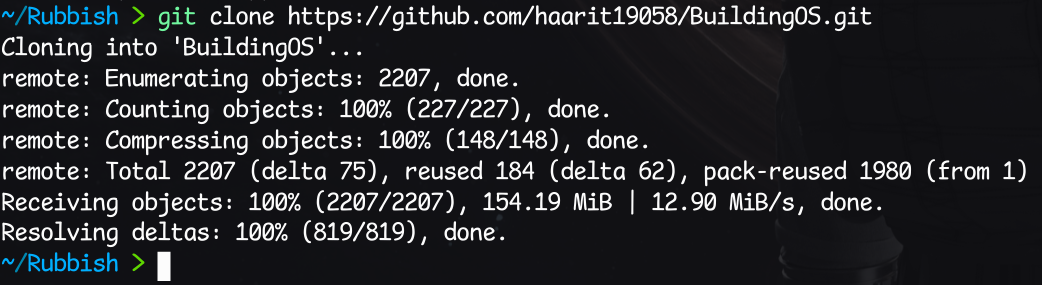
\includegraphics[width=0.75\linewidth]{image11.png}
    \caption{Cloning a repo}
    \label{fig:placeholder}
\end{figure}


To get the code from remote repo execcute this command : git pull origin main
\begin{figure}[H]
    \centering
    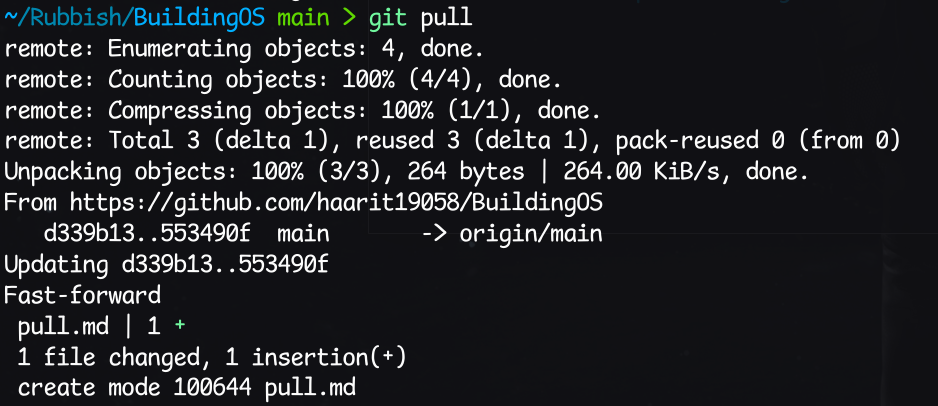
\includegraphics[width=0.75\linewidth]{image12.png}
    \caption{Pull from remote}
    \label{fig:placeholder}
\end{figure}


Now that Lab 01 has reached its midway point, it's time to set up GitHub Actions—one of the most exciting and productive features of GitHub. We'll integrate Pylint with GitHub Actions to automatically check code quality on every push or pull request.

Pylint is a static code analysis tool for Python that examines source code without executing it. It helps developers identify errors, enforce coding standards based on PEP 8, and provides suggestions for refactoring and improving code consistency. Using Pylint is ideal for keeping code reliable, readable, and maintainable throughout a project's lifecycle.

For any workflow on GitHub we need to add a YAML file corresponding to that particular action in \texttt{.github/workflow/actionname.yaml}. By using the GUI as shown below we will add pylint to our repository.


\begin{figure}[H]
    \centering
    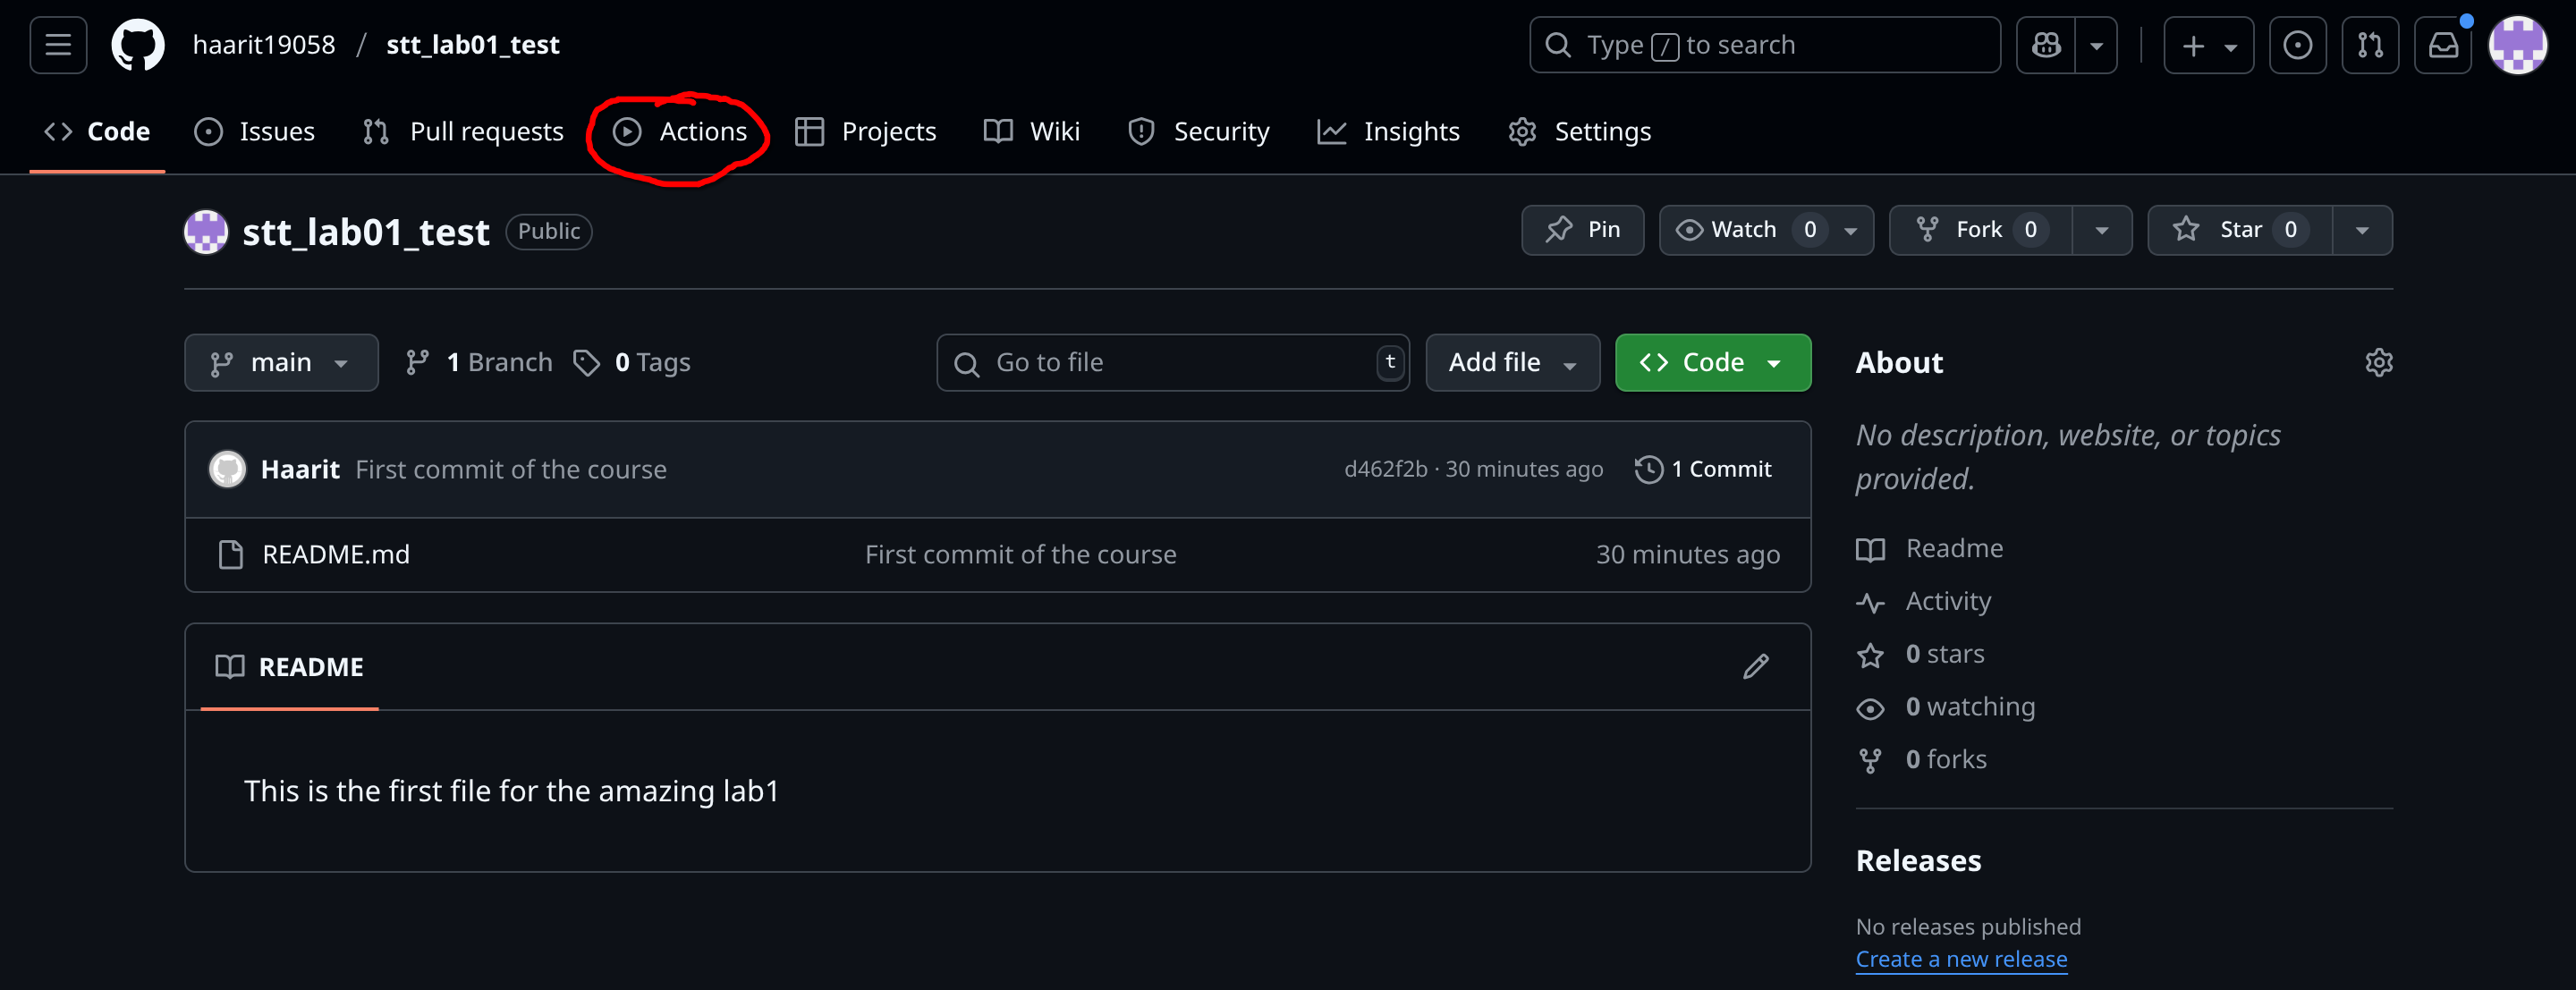
\includegraphics[width=0.75\linewidth]{image13.png}
    \caption{Navigating to Github actions}
    \label{fig:placeholder}
\end{figure}

\begin{figure}[H]
    \centering
    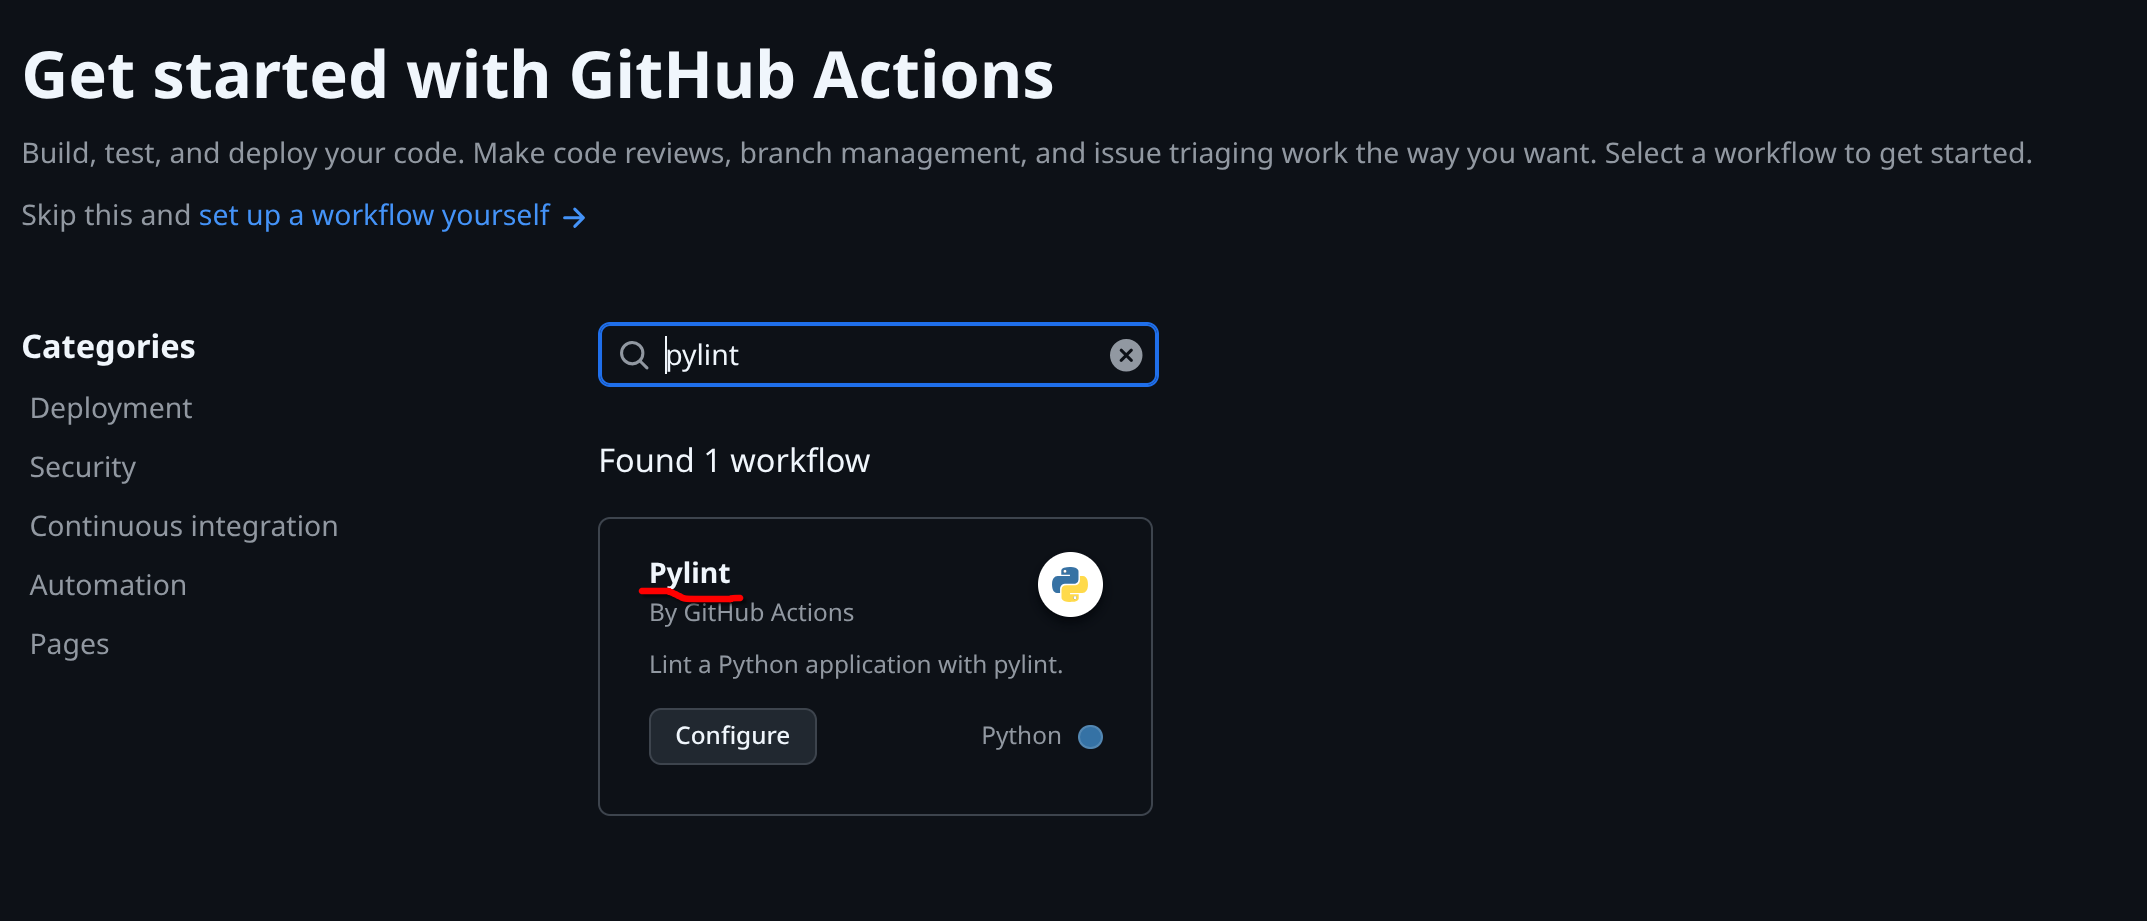
\includegraphics[width=0.75\linewidth]{image14.png}
    \caption{Finding pylint}
    \label{fig:placeholder}
\end{figure}

\begin{figure}[H]
    \centering
    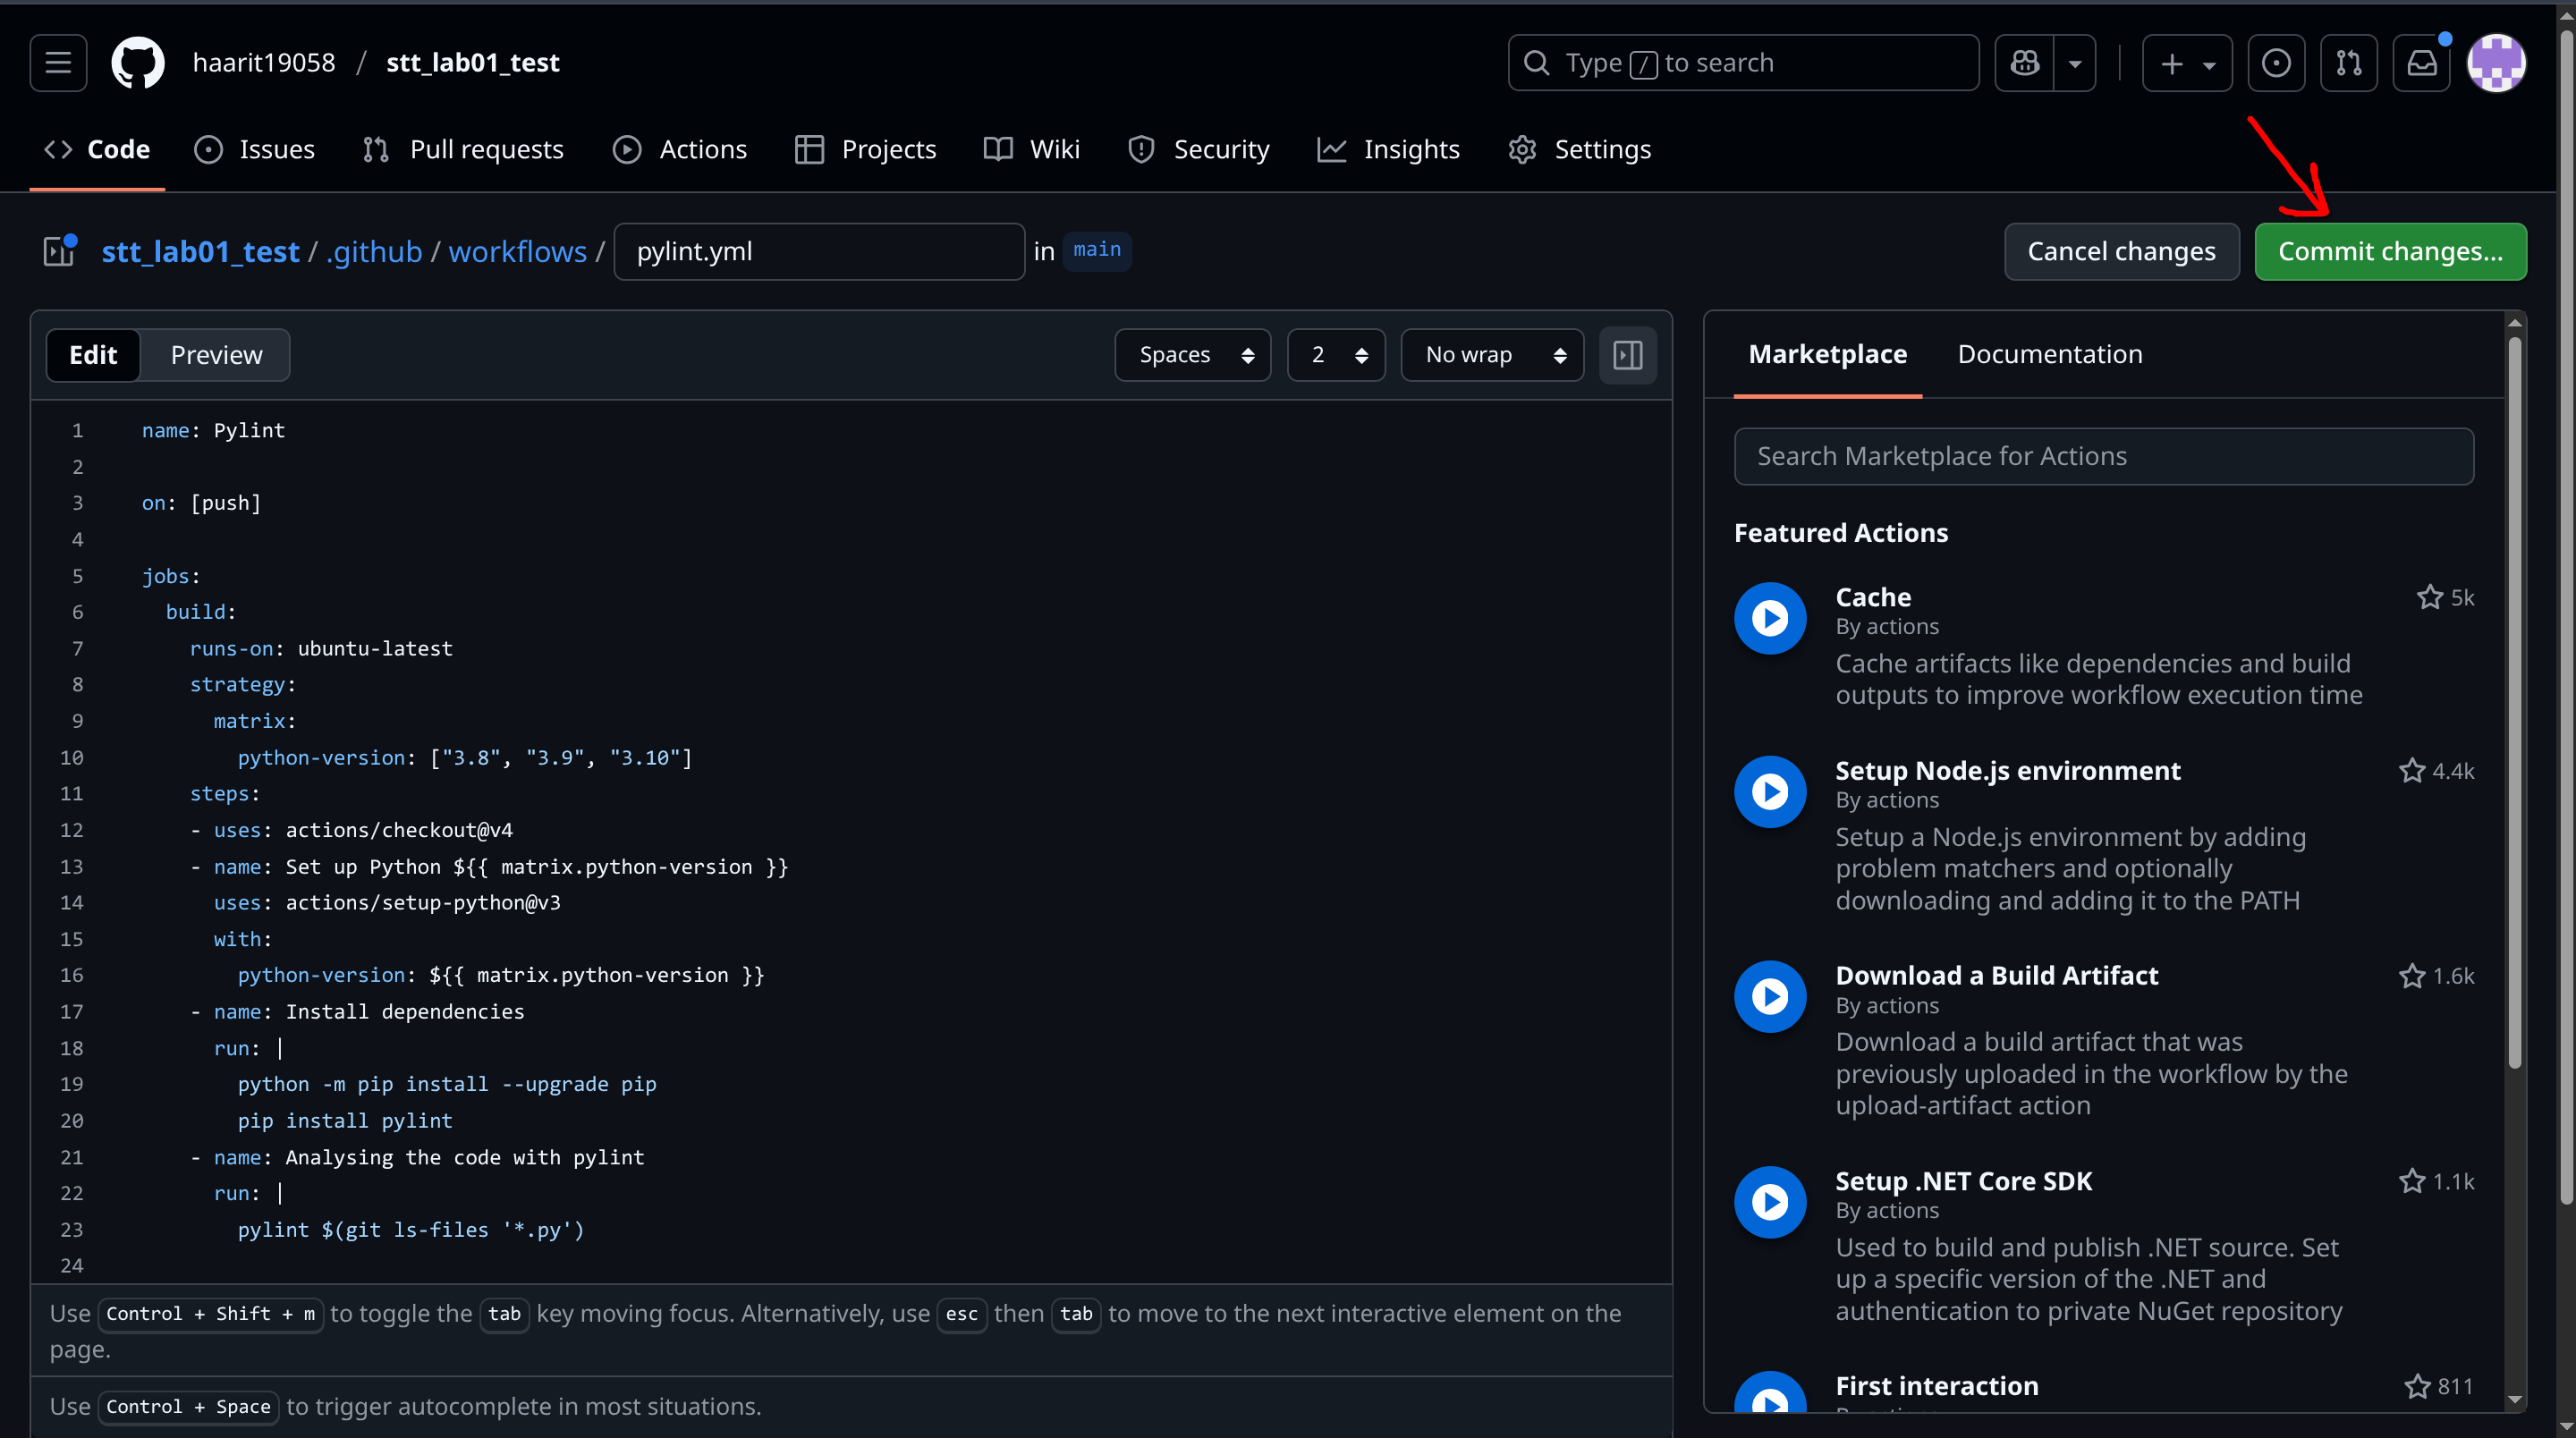
\includegraphics[width=0.75\linewidth]{image15.png}
    \caption{Commit changes .github/workflows/pylint.yaml}
    \label{fig:placeholder}
\end{figure}

\subsection{Result and Analysis}

I have added a hello.py where i have implemented sudoku solver in python and pushed the changes to remote repo. It automatically runs the pylint and this is the output ..
\begin{figure}[H]
    \centering
    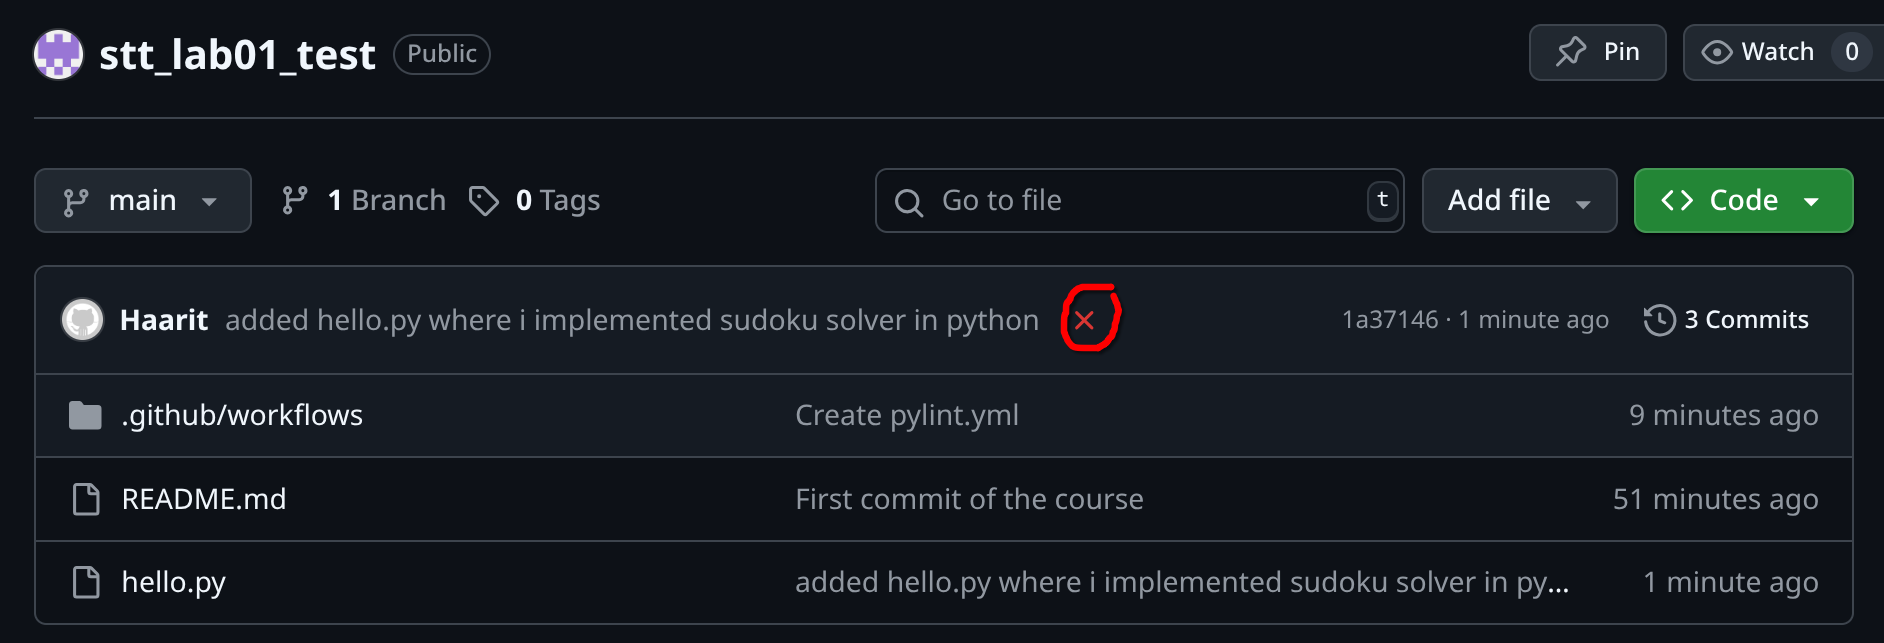
\includegraphics[width=0.75\linewidth]{image16.png}
    \caption{pylint on hello.py}
    \label{fig:placeholder}
\end{figure}

pylint runs a lots of checks on the code here is the analysis for this commit ..
\begin{figure}[H]
    \centering
    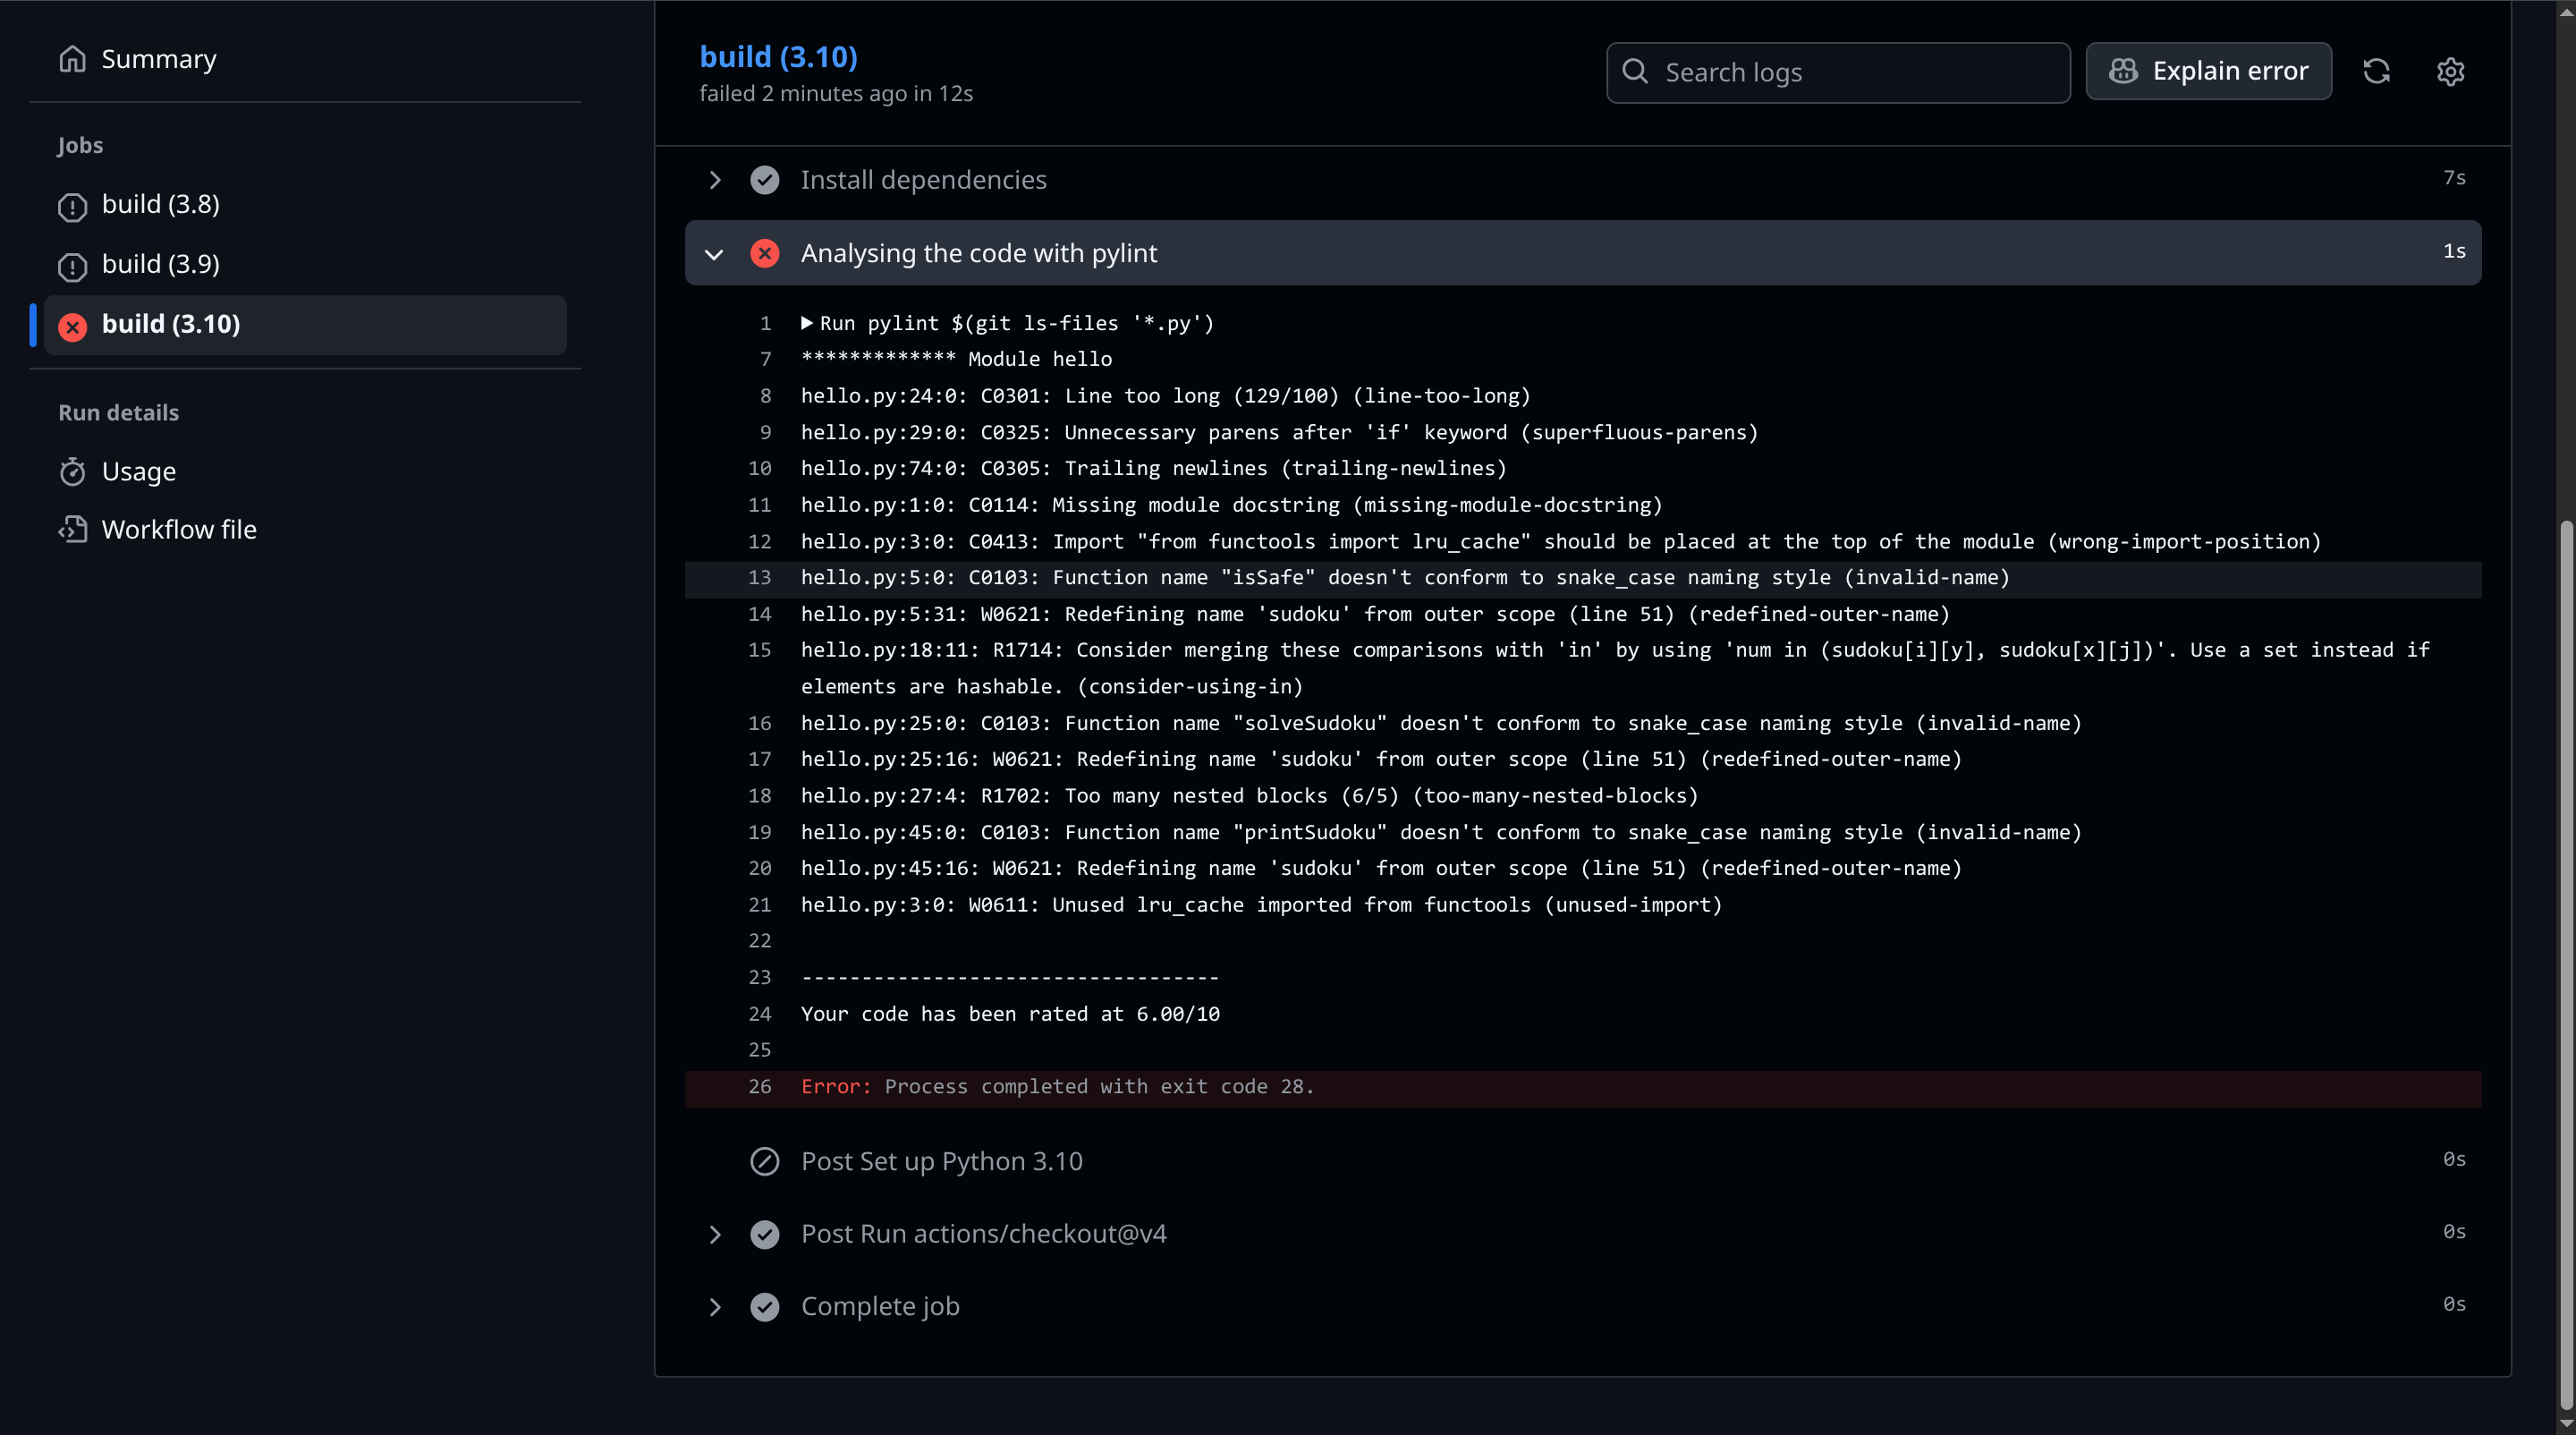
\includegraphics[width=0.75\linewidth]{image17.png}
    \caption{Pylint analysis}
    \label{fig:placeholder}
\end{figure}

Now, i have fixed the hello.py by removing multiple nested for loops and adding comments for functions and the overall score given by pylint has increased.

\begin{figure}[H]
    \centering
    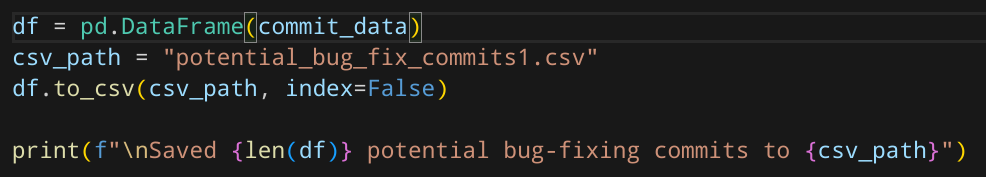
\includegraphics[width=0.75\linewidth]{image.png}
    \caption{Satifying the criteria of pylint}
    \label{fig:placeholder}
\end{figure}



\subsection{Discussion and Conclusion}
Overall, this lab highlighted the importance of version control and automation in modern software workflows. The skills learned here will enable developers to manage projects more effectively, maintain high-quality codebases, and streamline development processes through continuous integration and deployment practices. These practices are essential for professional software development and collaboration in both academic and industry settings.

\subsection{References}
\begin{enumerate}
    \item Lecture Slides
    \item \href{https://education.github.com/git-cheat-sheet-education.pdf}{GitHub Git Cheat Sheet (PDF)}
\end{enumerate}



\newpage
\section{Lab 02}
\subsection{Introduction and Concepts}
This lab aims to teach the fundamentals of mining open source software (OSS) repositories. It involves processing and analyzing commits from the GitHub version control system for widely used real-world projects. In practice, the definition of a bug and its fix is best determined by the developers contributing to those projects. Existing tool may struggle to capture project specific or domain specific semantics. The primary goal of this lab assignment is to develop a framework for understanding how developers perceive bug-fixing commits.
\subsection{Tools and Setup}
\begin{itemize}
    \item Torch: A framework for running machine learning models efficiently.
    \item Transformers: A library designed for working with large language models (LLMs) and natural language processing tasks.
    \item PyDriller: A tool that traverses GitHub repositories commit by commit and provides a convenient API for mining software repository data.
    \item Pandas: A library for handling and analyzing data, useful for working with CSV files.
    \item Anaconda: A tool for managing Python environments and packages.
    \item SEART :  search engine for github repositories
\end{itemize}

Creating a new environment and installing necessary packages :
\begin{itemize}
    \item conda create --name pystt python=3.12
    \item pip install torch transformers pydriller pandas 
\end{itemize}

\subsection{Methodology and Execution}

First we have to select a repository that we will be using thorughout the assignment. For that we will use SEART for searching github repos. I put the following criteria :
\begin{itemize}
    \item stars >= 10k
    \item commits >= 1000
    \item language == python
    \item the project must be well known and used by many
\end{itemize}

\begin{figure}[H]
    \centering
    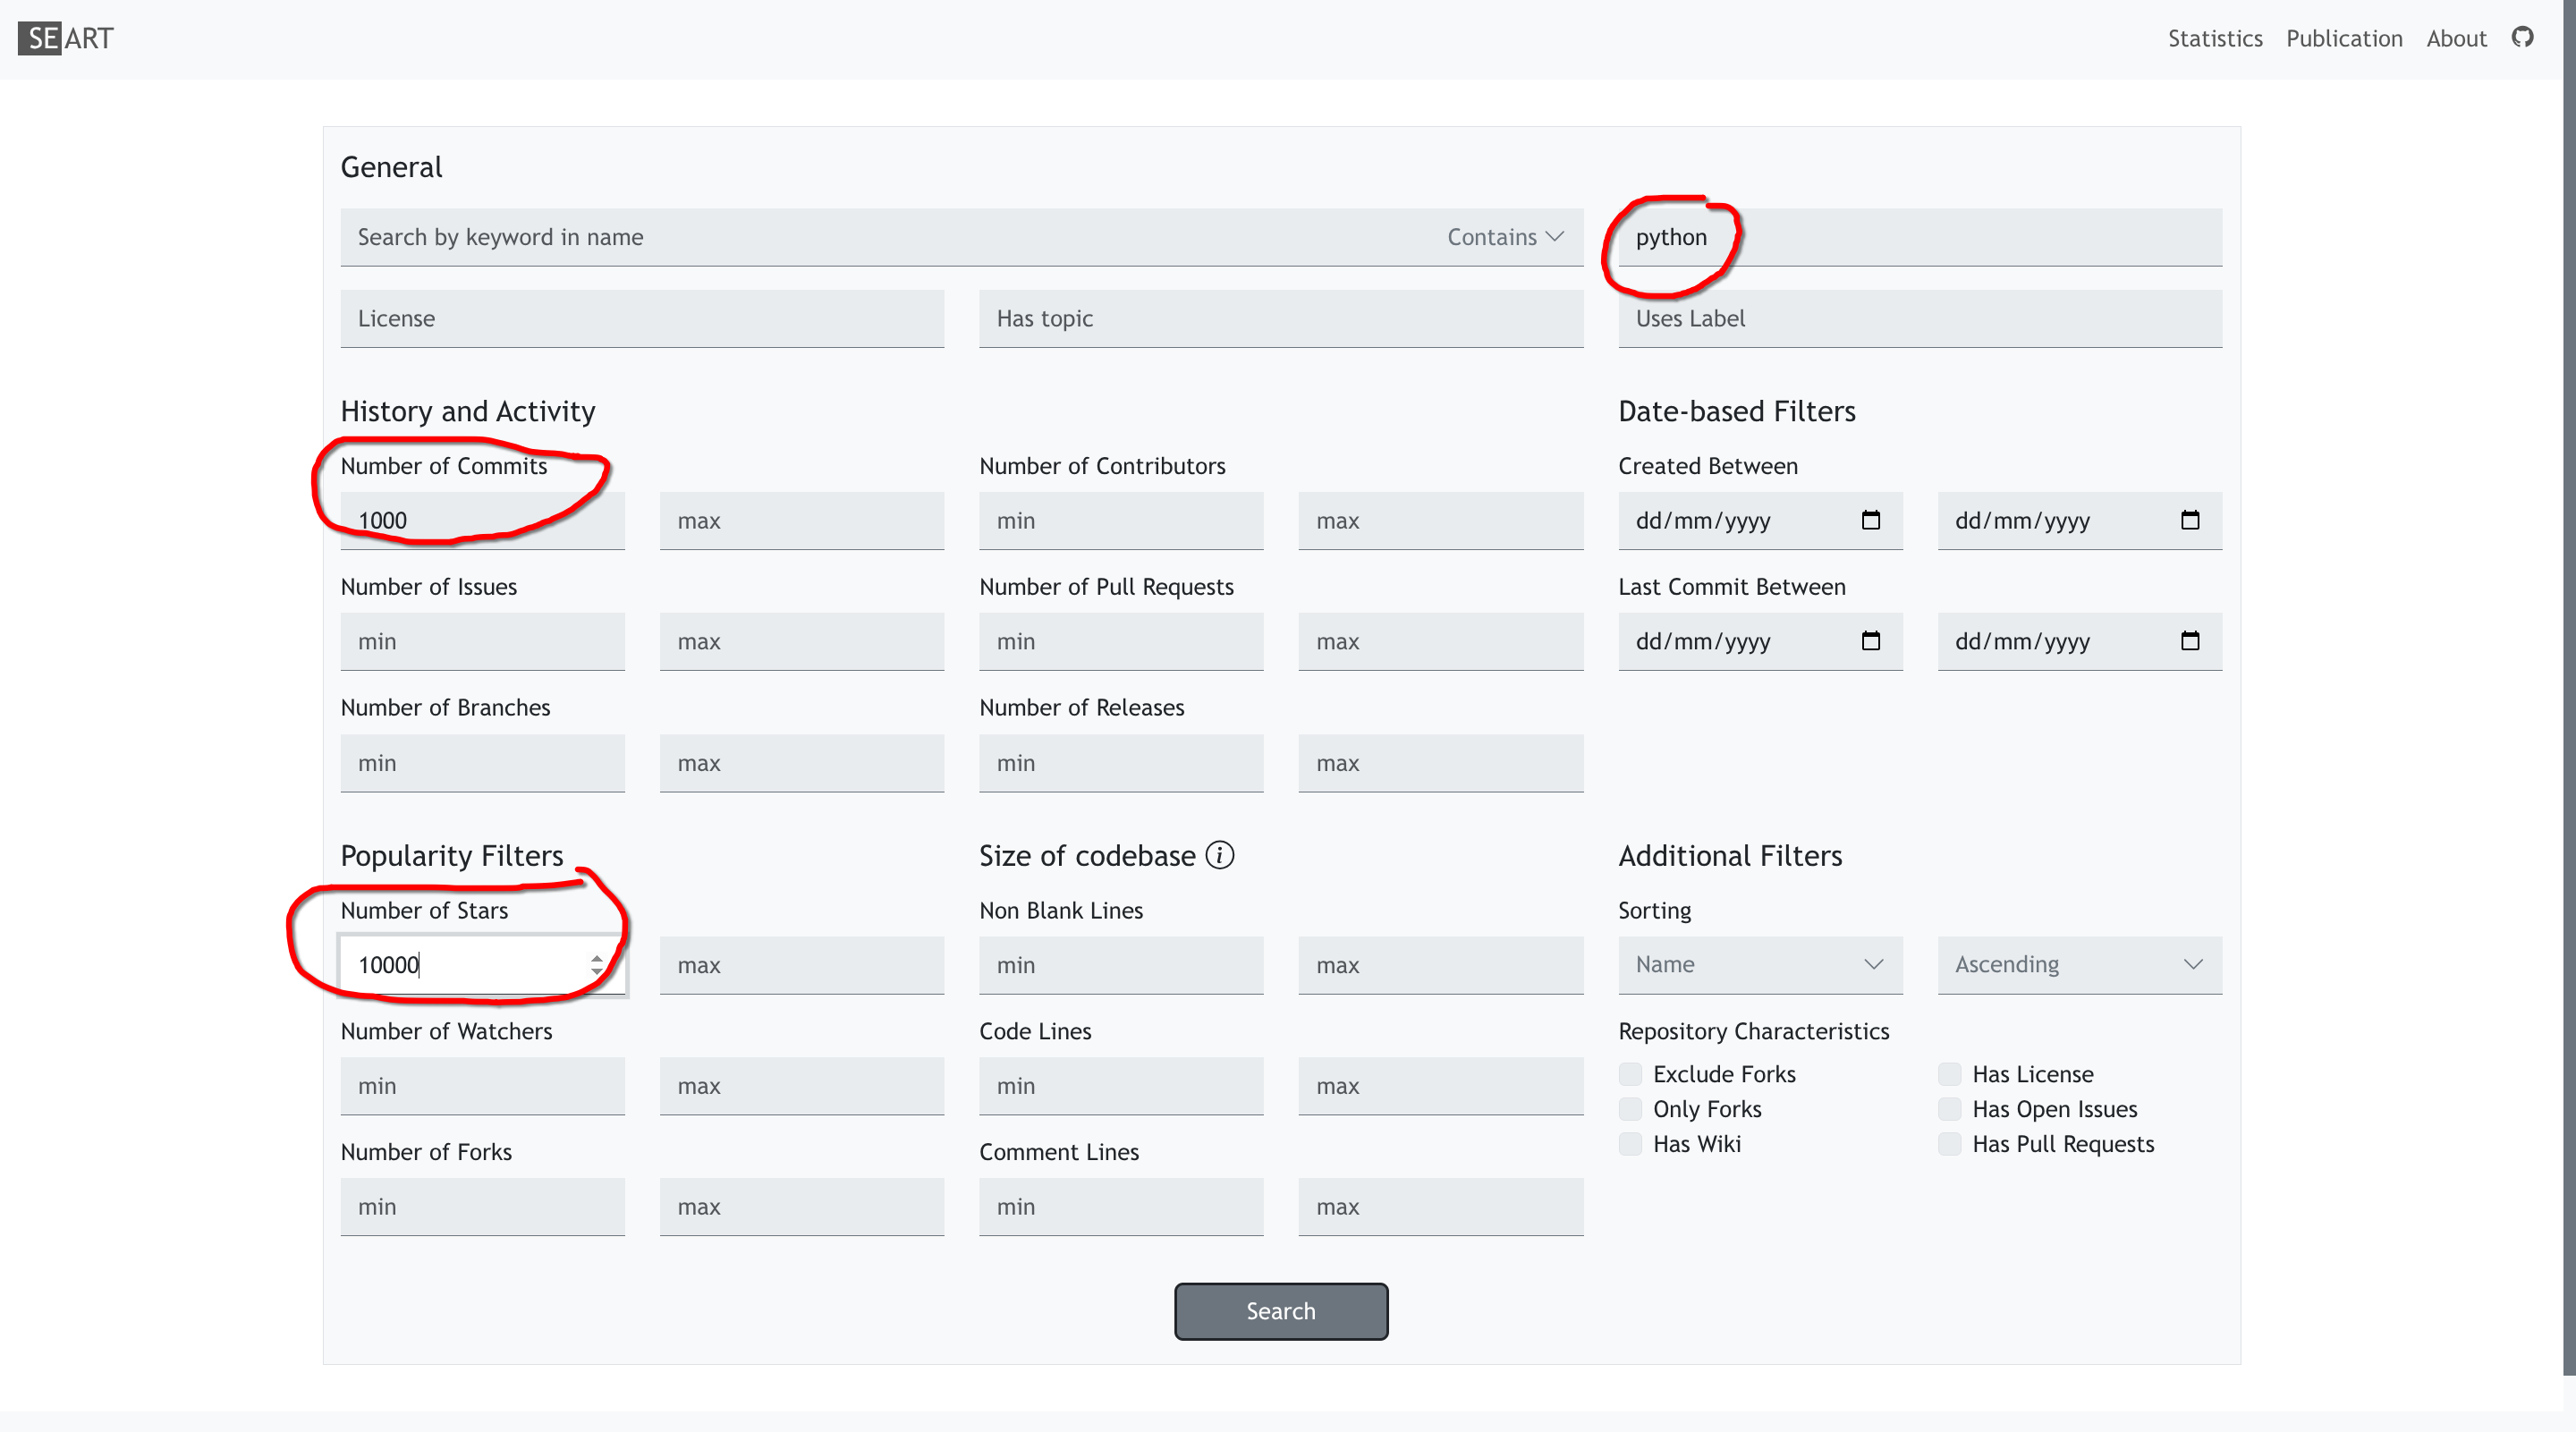
\includegraphics[width=0.75\linewidth]{image18.png}
    \caption{SEART}
    \label{fig:placeholder}
\end{figure}

So from the results I read through few of the repos and finally decided to work upon agno. Agno is a full-stack framework for building Multi-Agent Systems with memory, knowledge and reasoning. Here is the link to repository : \href{link}{https://github.com/agno-agi/agno.git}. 

Now moving on to the next part we need to identify which commits are bug fixing commits. For that i use the straight forward approach of checking whether the commit message by developer contains certian set of words like "fix" or "bug". If the message contains such words then classify it as bug fixing commit and store the data into the table.

Here are the words that i took from the lecture slides to identify bug fix commits :
\begin{figure}[H]
    \centering
    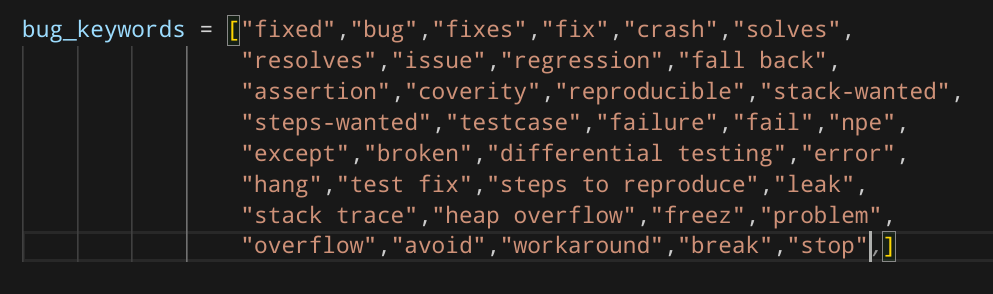
\includegraphics[width=0.75\linewidth]{image19.png}
    \caption{Bug - Keywords}
    \label{fig:placeholder}
\end{figure}

This is the function to check whether a message is bug-fix message or not.
\begin{figure}[H]
    \centering
    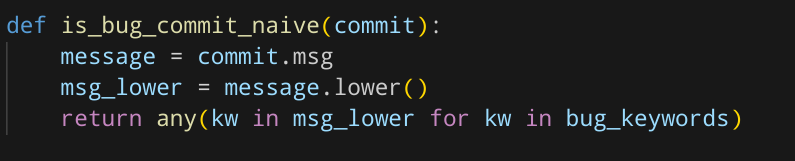
\includegraphics[width=0.75\linewidth]{image20.png}
    \caption{bug_fix_naive}
    \label{fig:placeholder}
\end{figure}

Now we use the API provided by pydriller to traverse the commit and store the necessary information in a list if the commit is bug fixing commit.
\begin{figure}[H]
    \centering
    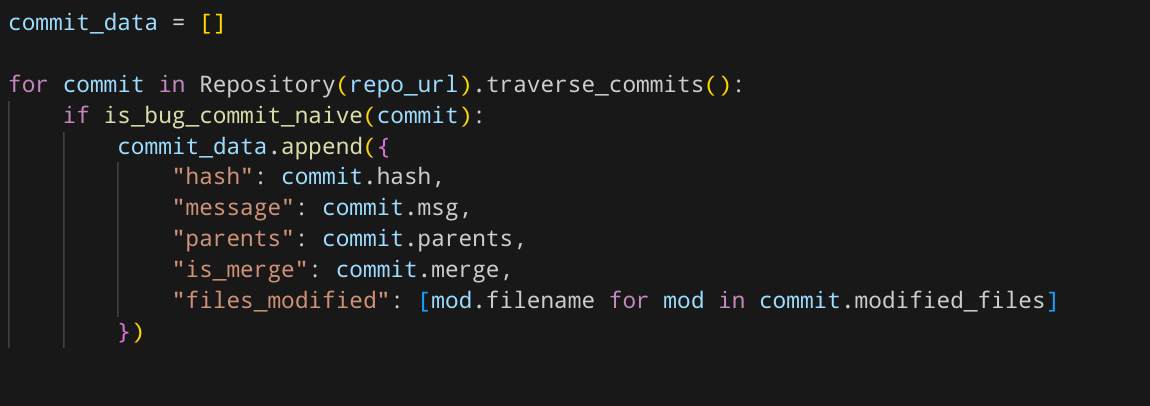
\includegraphics[width=0.75\linewidth]{image21.png}
    \caption{traverse using pydriller}
    \label{fig:placeholder}
\end{figure}

Now we will store the data into a csv file as required in the assignment.
\begin{figure}[H]
    \centering
    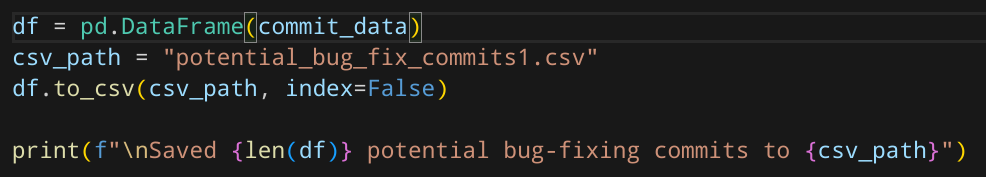
\includegraphics[width=0.75\linewidth]{image.png}
    \caption{store into csv}
    \label{fig:placeholder}
\end{figure}

Now moving on to diff extraction and analysis part. As mentioned in the assignment we will use the llm to generate tags on per file basis. First we will load the model and then add a new field in the previous code for llm inferencing.


The function to do inference and setting up the model.
\begin{figure}
    \centering
    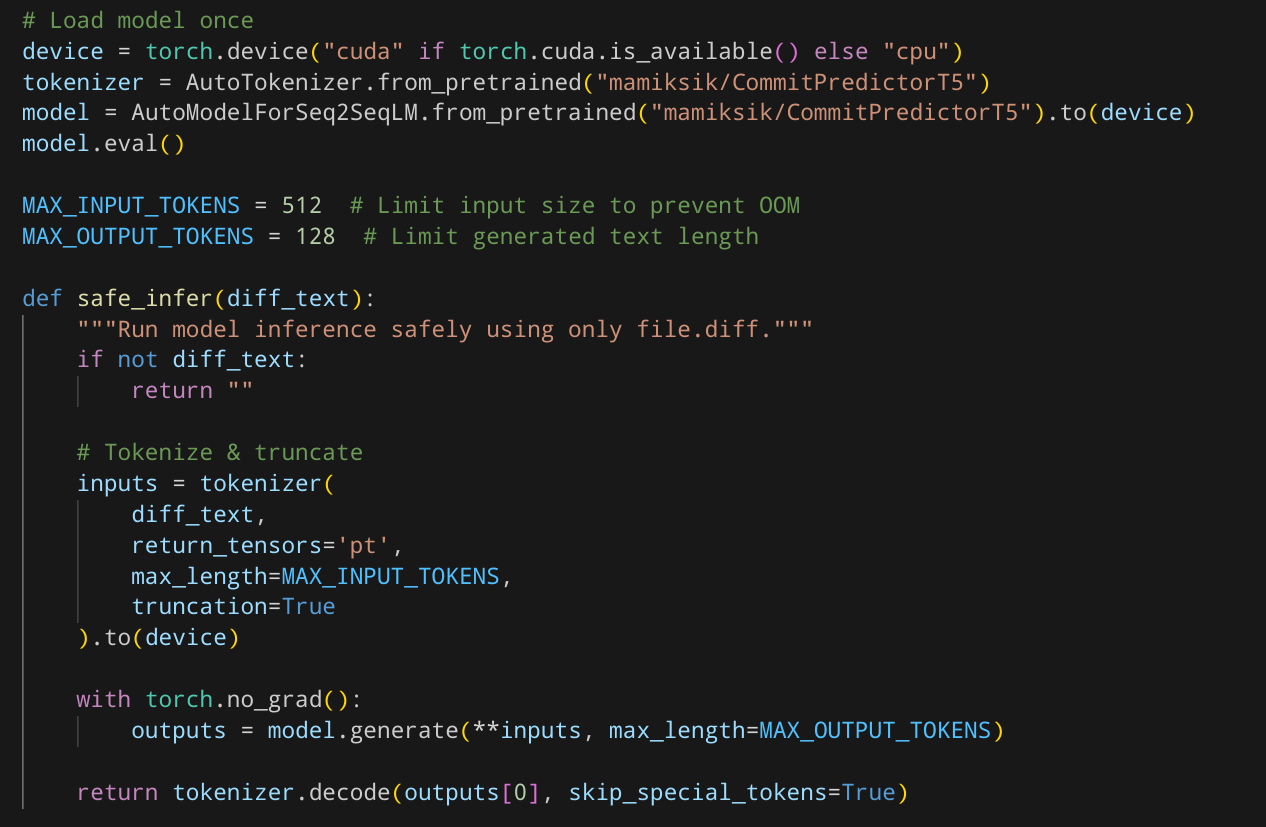
\includegraphics[width=0.75\linewidth]{image22.png}
    \caption{inference function}
    \label{fig:placeholder}
\end{figure}



\begin{figure}
    \centering
    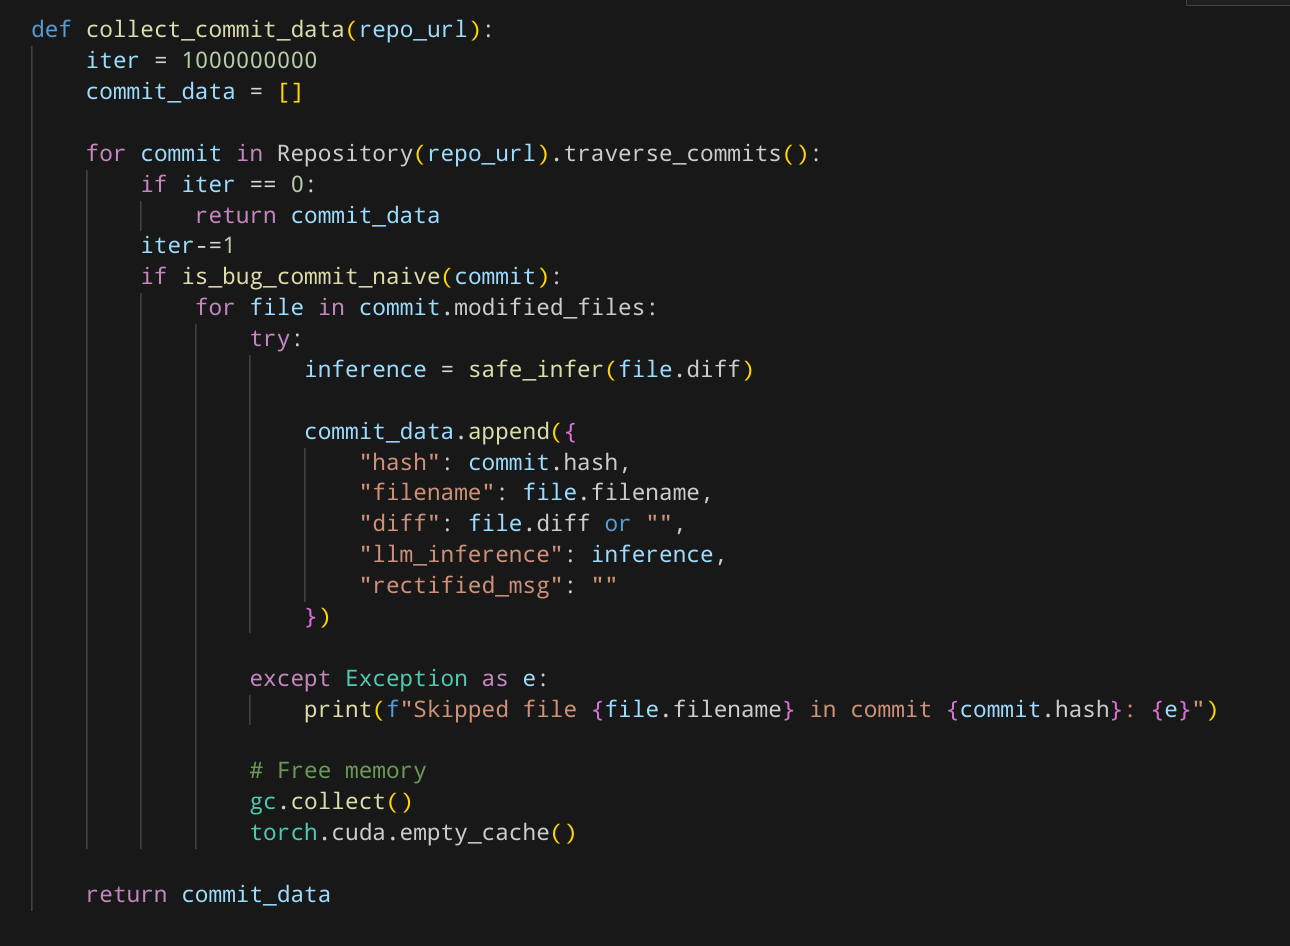
\includegraphics[width=0.75\linewidth]{image23.png}
    \caption{llm inference code}
    \label{fig:placeholder}
\end{figure}


\textbf{Rectifier Formulation}

This is an open ended task so there are many ways to make a rectifier. My approach is as follows:
\begin{itemize}
    \item First collect the per file tags by the given llms
    \item use llama-3-8b model using groq api 
    \item Make a prompt that gives data as file : llm tag and ask llama to create a commit message based on this data.
\end{itemize}

I also tried to generate a commit message by passing the file diffs to the model but it reached the token limit and due to resource constraint next best option that i found feasible is to give file and llm\_tags to model.

Funtion to get response from llama given the data
\begin{figure}
    \centering
    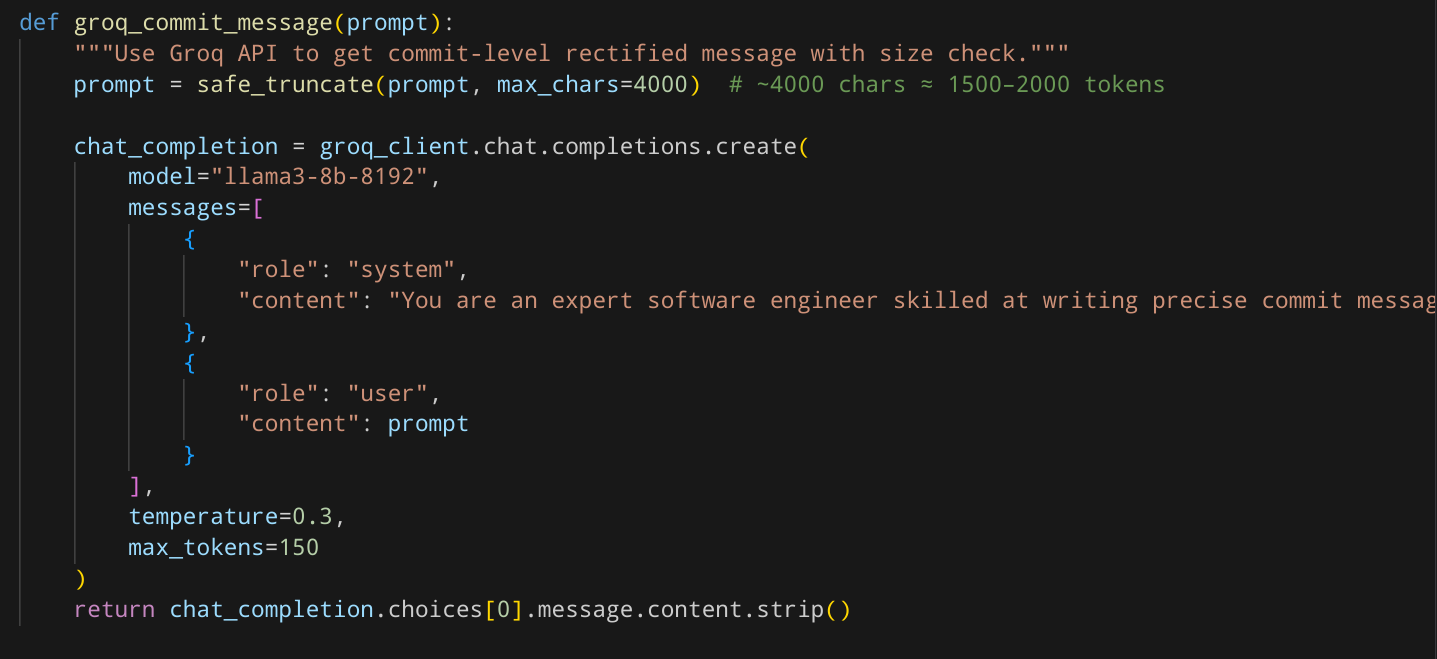
\includegraphics[width=0.75\linewidth]{image24.png}
    % \caption{}
    \label{fig:placeholder}
\end{figure}


Now we will integrate this to previous code so that we can make a final file that contains the data as a single table as asked in assignment.
\begin{figure}
    \centering
    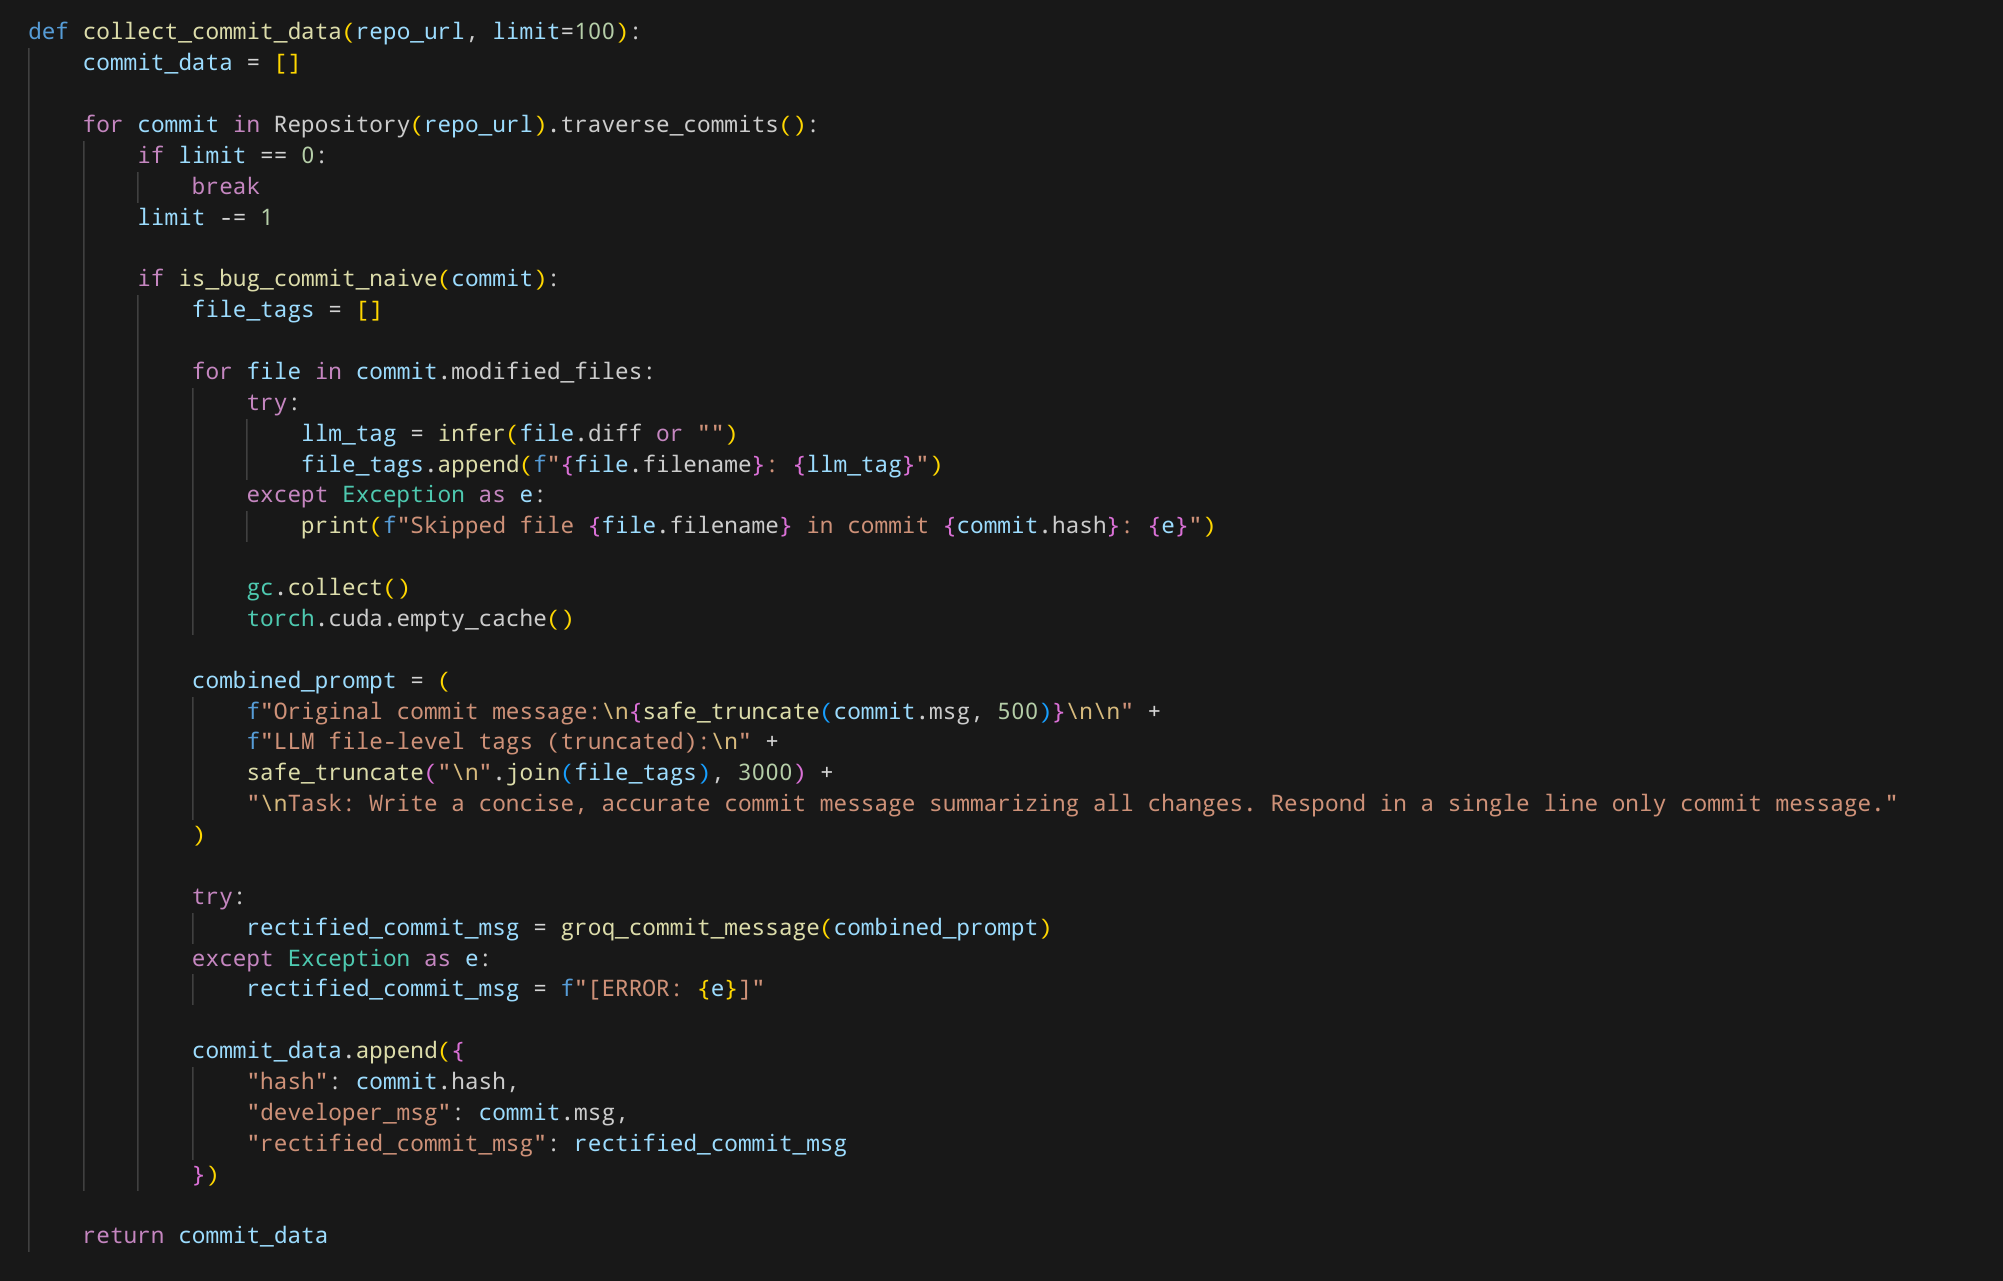
\includegraphics[width=0.75\linewidth]{image25.png}
    \caption{integrating groq}
    \label{fig:placeholder}
\end{figure}


% evaluation research question remaining
\subsection{Result and Analysis}
After running the code it will create a file named master\_commits.csv that contains data as asked.

Lets take a single entry from the file to see the final result.
Commit Hash : 886f0a4e876cd38f7611afba273bf485eed6c605
Developer Message : Fix formatting
Rectified Message : Refactor code formatting and add missing documentation and examples across multiple files for improved readability and usability.

Files changed and llm tag:
README.md 
assistant.py 
assistant_stream_off.py 
cli.py 
pydantic_output.py 
tool_call.py 
arxiv_kb.py 
pdf.py 
website.py 
wikipedia_kb.py 
__init__.py 
openai_chat.py 
__init__.py 
chat.py

\subsection{Discussion and Conclusion}
\subsection{References}

\newpage
\section{Lab 03}
\subsection{Introduction and Concepts}
\subsection{Tools}
\subsection{Setup}
\subsection{Methodology and Execution}
\subsection{Result and Analysis}
\subsection{Discussion and Conclusion}
\subsection{References}

\newpage
\section{Lab 04}
\subsection{Introduction and Concepts}
\subsection{Tools}
\subsection{Setup}
\subsection{Methodology and Execution}
\subsection{Result and Analysis}
\subsection{Discussion and Conclusion}
\subsection{References}




\newpage
% Appendixes
\appendix
\section{Appendix}
\begin{figure}[!ht]
    \centering
    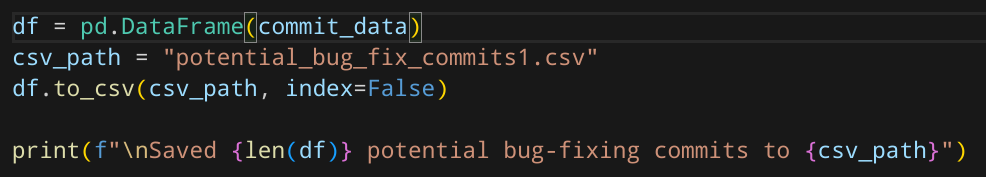
\includegraphics[width=\textwidth]{image.png}
    \caption{Caption of the photo.}
    \label{fig:myimage}
\end{figure}

% Bibliography
\clearpage
\pagestyle{\auxsettings}
\printbibliography[heading=bibintoc]
\end{document}






























% all in one template is the name of this shit



% %%% Here is the class with everything we need, if you don't want, you don't have to take a look at it, as it will probably cover your needs by far. These three options are used after the class article, which this template is based in.
% % Twoside will act as an special parameter, because if the document is twosided indeed, headers and footers will be adapted in consequence.
% % I recently added the language parameter to change it more easily, so the label of all theorems are redefined accordingly, depending on which is used. Disclaimer: only available for Catalan, English and Spanish. If no language is selected, English is enforced.


% % \documentclass[a4paper,12pt,oneside,catalan]{all-in-one} %% ONESIDE
% \documentclass[a4paper,12pt,twoside,english]{all-in-one} %% TWOSIDE

% % Here is the font I usually use, it can be changed of course.
% % In that case, these next two lines have to be deleted.
% \usepackage{ebgaramond}
% % Equations have the same font.
% \usepackage[cmintegrals,cmbraces,ebgaramond]{newtxmath}

% \doctitle{Subject}
% \docsubtitle{Document Title}

% \author{Author 1 \\ \texttt{ID} \and Author 2 \\ \texttt{ID} \and Author 3 \\ \texttt{ID} \and Author 4 \\ \texttt{ID}}

% % A text that goes into the footer. You can even include a logo. It can be left blank, too.
% %% Option 1: \footext{
\includegraphics[width=2em]{titlepage.png}}
% %% Option 2: \footext{\copyright\ \the\year by Cookie Monster}
% % What I usually use: 
% \footext{}

% % Don't comment the command below if it's not of much inconvenience, please!
% \greetings
% % Licensing on every page? Comment if you don't want it.
% % \licensing

% % Last things
% % This is my favourite config for bibliography. Each one of the references can be briefly explained with the field "note".
\RequirePackage[style=english]{csquotes}
\RequirePackage[
backend=biber,
style=alphabetic,
sorting=ynt
]{biblatex}
\newcommand{\familynameformat}[1]{\MakeUppercase{#1}}
\AtBeginBibliography{%
  \renewcommand{\mkbibnamefamily}{\familynameformat}%
}
\renewbibmacro*{begentry}{%
  \iffieldundef{note}
    {\undef\bbxnote}
    {\savefield{note}{\bbxnote}%
     \clearfield{note}}}
\renewbibmacro*{finentry}{%
  \restorefield{note}{\bbxnote}%
  \iffieldundef{note}
    {\finentry}
    {\setunit{\finentrypunct\par\vspace{\bibitemsep}\nobreak}
     \textit{\printfield{note}}%
     \finentry}}
\let\familynameformat=\textsc
\nocite{*}

\addbibresource{bibl.bib}


% Hyperref always required last one.
\RequirePackage{hyperref}
\makeatletter
\hypersetup{%
  hidelinks,
  pdfstartview=Fit,%
  pdfmenubar=true,%
  pdftoolbar=true,%
  bookmarksopen=false,%
  pdftitle={\@docsubtitle},%
  pdfauthor={\templateauthor},%
  pdfsubject={\@doctitle},%
  pdflang={\languagename},%
  pdfkeywords={mathematics},%
  pdfproducer={pdfTeX}}
\makeatother

% Setting up the titlepage.
\makeatletter%
\title{{\large\textit{\@doctitle}}\\[0.5cm]{\Huge\color{gray}\textsc{\@docsubtitle}}}%
\makeatother%
\date{\today}

% % Dummy text
% \usepackage{lipsum}

% \begin{document}
% % Interlineate, it can be changed.
% \setlength{\baselineskip}{.70cm}

% \begin{titlepage}
% \maketitle\vfill
% \centering
\includegraphics[width=20em]{titlepage.png}
% \doclicenseThis
% % Very important, regarding page numbering. Keep in mind differences between oneside and twoside
% \thispagestyle{empty}
% \end{titlepage}

% % Table of contents
% \thispagestyle{plain}
% \tableofcontents
% \newpage

% \pagestyle{\defaultsettings}

% \section{Introduction}
% \lipsum[1-3]
% \begin{equation}\label{eq:hello}
%     \frac{\partial f}{\partial x}(x,y)=\text{hello}
% \end{equation}
% \subsection{Subsection}
% \lipsum[4-8] \eqref{eq:hello}
% \section{Other}
% \lipsum[10-13]
% \section{Another}
% \begin{enumerate}
%     \item \lipsum[14]
%     \item \lipsum[15]
% \end{enumerate}

% % Theorem environments
% \begin{theorem}
% \lipsum[16]
% \end{theorem}
% \begin{proof}
% \end{proof}
% \begin{corollary}
% \lipsum[16]
% \end{corollary}
% \begin{definition}
% \lipsum[16]
% \end{definition}
% \begin{remark}
% \lipsum[16]
% \end{remark}
% \begin{exercise}
% \lipsum[16]
% \end{exercise}
% \begin{proof}[Solution]
% \lipsum[17]
% \end{proof}
% \clearpage

% % Appendixes
% \appendix
% \section{Appendix}
% \begin{figure}[!ht]
%     \centering
%     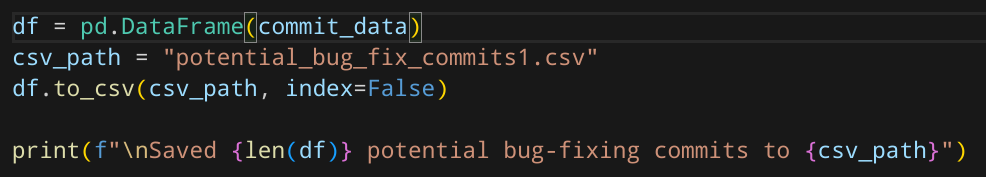
\includegraphics[width=\textwidth]{image.png}
%     \caption{Caption of the photo.}
%     \label{fig:myimage}
% \end{figure}

% % Bibliography
% \clearpage
% \pagestyle{\auxsettings}
% \printbibliography[heading=bibintoc]
% \end{document}